%============================
% LifeV - State of the Art
% July 2010
%
% Author: Gwenol Grandperrin <gwenol.grandperrin@epfl.ch>
%
% Contributors:
% Paolo Crosetto
% Simone Deparis
% Gilles Fourestey
% Cristiano Malossi
% Samuel Quinodoz
% Ricardo Ruiz
% Paolo Tricerri
%============================

\documentclass[11pt]{article}

\usepackage{amssymb}
\usepackage{amsmath}
\usepackage{float}
\usepackage{pifont}
\usepackage{graphicx}
\usepackage{subfigure}
\usepackage{algorithme}
\usepackage{longtable}
\usepackage{eqnarray}

%Pour aligner verticalement les tableaux
\usepackage{array}
\newcolumntype{M}[1]{>{\centering}m{#1}}

\newcommand{\tick}{\ding{51}}

\newcommand{\norm}[1]{\left\| #1 \right\|}

\begin{document}
\title{LifeV - State of the Art}
\author{Gwenol Grandperrin, Paolo Crosetto, Simone Deparis,\\
	Gilles Fourestey, Cristiano Malossi, Samuel Quinodoz, \\
	Ricardo Ruiz, Paolo Tricerri}
\date{\today}
\maketitle

%============================
% Introduction
%============================
\section{Introduction}
%LifeV is a finite element (FE) library.
Nowadays super computers had become very efficient. However solving huge systems still requires research and development of efficient tools. One can think for example of the simulation of the entire cardiovascular system. To face such kind of challenges, the CMCS at EPFL in Switzerland, the MOX at Politechnico di Milano in Italy and REO group at INRIA in France have developed a C++ 3D finite element code called LifeV (prononced "life-five"). In 2006, CMCS started to parallelize the library.

In this document we describe the actual level of both knowledge and development of LifeV. The content is actually made of contributions of the developers themselves.

In Section~\ref{sec:lifev} we will describe the core of the library, i.e., the solvers, the finite elements, the boundary conditions and the tools available. Then in Section~\ref{sec:applications}, we present the current applications done with LiveV. Finally in the Section~\ref{sec:otherProjects}, one can find other projects where the LiveV library was one of the key aspect.

%============================
% LifeV, a Finite Elements library
%============================
\section{LifeV, a C++ finite element library}
\label{sec:lifev}

As mentioned in the introduction, LifeV is a finite element library which has been implemented in C++. The development started in 2002 and the code contains today around 50.000 lines. The code is free and available on http://www.lifev.org under LGPL license.

In 2010, a new release of the code has been proposed where the whole code has been ported to a parallel version to achieve high performance computing on multiprocessors architectures. The largest number of degrees of freedom computed in a simulation with the new version is nine  millions. All the efforts are now made to prepare LifeV for the architectures of tomorrow's supercomputers.
% Note: the nine millions of DOF has been done with an ethiersteinman problem by Gilles Fourestey

In Section~\ref{sec:solvers}, we describe first the physical solvers implemented in LifeV. Then we present the finite elements, the boundary conditions and the input/output management in Sections~\ref{sec:BC}, \ref{sec:FE} and \ref{sec:inOutput} respectively.

% Solvers available in LifeV
\subsection{Physical solvers available in LifeV}
\label{sec:solvers}
We refer to a physical solver class as a class that is able to build the discrete system associated to the approximation of a PDE.

In this section, we go through the existing physical solvers in LifeV. Hence the reader will have a clear idea of the possible equations which can be solved.

%\subsubsection{Harmonic Extension solver}
\subsubsection{HarmonicExtensionSolver class}
This solver deals with the Laplace equation:
\begin{eqnarray}
\Delta\eta & = & 0\\
+\text{b.c.}\nonumber
\end{eqnarray}
 However more features have been implemented to use it as a tool in the Arbitrary Eulerian Lagrangian (ALE) framework (more informations can be found in~\cite{nobile} or~\cite{quarteroni}). The harmonic extension technique allows  for example to move the points of a mesh in the latter framework.

The following table gives an overview of the main methods available in the HarmonicExtensionSolver class:

%\begin{table}[H]
\begin{center}
\begin{longtable}{p{3cm}p{7cm}}
	\hline
	\texttt{setUp(dataFile)} & Sets up the system solver with a GetPot datafile\footnote{GetPot is a parsing configuration files library available at http://getpot.sourceforge.net}\\
	\texttt{initialize(disp)} & Initialization of the problem\\
	\texttt{buildSystem()} & Builds the system\\
	\texttt{updateSystem()} & Stores the displacement value in the old displacement variable\\
	\texttt{iterate(BCHandler)} \\
	& Updates the convective term, does the boundary conditions treatment and solves the linear system.\\
	\texttt{dispOld()} & Returns the old value of the displacement\\
	\texttt{dispDiff()} & Displacement difference (between the old and the new displacement)\\
	\texttt{disp()} & Returns the displacement\\
	\texttt{setDisplacement(disp)} \\
	& Sets the value of the displacement with a vector\\
	\texttt{setDispOld(disp)} & Sets the value of the old displacement\\
	\texttt{getMap()} & Getter for the map\\
	\texttt{comm()} & Returns the MPI communicator\\
	\texttt{isLeader()} & Returns true on the Rank 0 process\\
	\texttt{resetPrec(bool)} & Resets the preconditioner of the linear solver\\
	\texttt{rescaleMatrix(dt)} & Multiplies the matrix by the scalar given as a parameter\\
	\texttt{applyBoundaryConditions(rhs,BCHandler)} \\
	& Applies the boundary conditions\\
	\texttt{computeMatrix()} & Computes the matrix of the system\\
	\texttt{updateDispDiff()} & Recomputes the value of the displacement difference\\
	\hline
\end{longtable}
\end{center}
%\caption{Main methods of the HarmonicExtensionSolver class}
%\label{tab:harmonicExtensionMethods}
%\end{table}

%\subsubsection{Oseen solver}
\subsubsection{Oseen class}
We consider a flow of an incompressible and viscous fluid decribed by its velocity $\mathbf{u}$ and its pressure $p$. We assume that the reynolds number is low. This solver is designed to get the solution of the so-called Oseen problem:
\begin{eqnarray}
\alpha\mathbf{u}+\boldsymbol{\beta}\cdot\nabla\mathbf{u}-\nu\Delta\mathbf{u} + \nabla p & = & f\\
\nabla\cdot\mathbf{u} & = & 0\\
+\text{b.c.}\nonumber
\end{eqnarray}
where $\nu=\frac{\mu}{\rho}$ is the kinematic viscosity of the fluid, $\mu$ the viscosity, $\rho$ the density, and $\alpha$ and $\beta$ are two parameters.

The main methods of the class are given in the following table:

%\begin{table}[H]
\begin{center}
\begin{longtable}{p{3cm}p{8cm}}
	\hline
	\texttt{iterate(BCHandler)} \\
	& Updates the convective term, does the boundary conditions treatment and solves the linear system.\\
	\texttt{updateSystem(alpha,beta,rhs,matrix)} \\
	& Updates the values of $\alpha$, $\boldsymbol{\beta}$, the rhs and the matrix \\
	\texttt{solution()} & Returns the local solution vector\\
	\texttt{residual()} & Returns the local residual vector\\
	\texttt{reduceSolution(u,p)} \\
	& Reduce the local solution into the global vectors for $\mathbf{u}$ and p\\
	\texttt{setSourceTerm(s)} & Sets the source term functor\\
	\texttt{sourceTerm()} & Returns the source term functor\\
	\texttt{post\_proc()} & Returns the Post Processing stuff.\\
	\texttt{area(flag)} & Computes the area on a given part of the boundary\\
	\texttt{flux(flag,vector)} & Computes the flux on a given part of the boundary\\
	\texttt{pressure(flag,vector)} \\
	& Computes the pressure on a given part of the boundary\\
	\texttt{LagrangeMultiplier(flag,BCHandler\_raw\_type)} \\
	& Gets the Lagrange multiplier related to a flux imposed on a given part of the boundary\\
	\texttt{flux(flag)} & Computes the flux on a given part of the boundary\\
	\texttt{pressure(flag)} & Computes the pressure on a given part of the boundary.\\
	\texttt{LagrangeMultiplier(flag)} \\
	& Gets the Lagrange multiplier related to a flux imposed on a given part of the boundary\\
	\texttt{postProcess(bool)} & Postprocessing\\
	\hline
\end{longtable}
\end{center}
%\caption{Main methods of the Oseen class}
%\label{tab:oseenMethods}
%\end{table}


%\subsubsection{Navier-Stokes solver}
\subsubsection{NavierStokesSolver class}
The classical Navier-Stokes equations for an incompressible viscous flow reads:
\begin{eqnarray}
\frac{d}{dt}\mathbf{u}+\mathbf{u}\cdot\nabla\mathbf{u}-\nu\Delta\mathbf{u} + \nabla p & = & f \label{eqn:NS1}\\
\nabla\cdot\mathbf{u} & = & 0\label{eqn:NS2}\\
+\text{b.c.}\nonumber
\end{eqnarray}
where $\mathbf{u}$ is the fluid velocity, $p$ the pressure, $\nu=\frac{\mu}{\rho}$ the kinematic viscosity of the fluid, $\mu$ the viscosity, $\rho$ the density and $f$ the external forces.

%The full implicit scheme is not yet implemented.
The table below gives an overview of the main methods of the class.

%\begin{table}[H]
\begin{center}
\begin{longtable}{p{3cm}p{8cm}}
	\hline
	\texttt{timeAdvance(source,time)} \\
	& Updates the right hand side for time advancing\\
	\texttt{iterate(time)} & Updates convective term, boundary conditions treatment and solve the linearized Navier-Stokes system\\
	\texttt{eval(fx0,gx0,x0,status)} \\
	& Sets the components of \texttt{fx0} relative to the degrees of freedom of $\mathbf{u}$ equal to the corresponding values of $\mathbf{u}$\\
	\texttt{initialize(x0,t0,dt)} \\
	& Initializes the values of the solution at the initial time step\\
	\texttt{initialize(string)} \\
	& Initializes the values of the solution at the initial time step with an external file\\
	\texttt{initializeNull()} & Initializes the values of the solution at the initial time step with a previously computed solution\\
	\texttt{initializeStokes(source,t0)} \\
	& Initializes with steady Stokes solution (without convection)\\
	\texttt{setUp(dataFile)} & Sets up the system solver with a GetPot datafile\\
	\texttt{buildSystem()} & Builds the matrix of the linear system\\
	\texttt{updateSystem()} & Updates the matrix of the linear system\\
	\texttt{u()} & Returns the solution for $\mathbf{u}$\\
	\texttt{p()} & Returns the solution for $p$\\
	\texttt{setFluidBC()} & Returns true if the boundary conditions are set\\
	\texttt{setFluidBC(BCHandler)} \\
	& Sets the fluid BCHandler\\
	\texttt{bcHandler()} & Returns the bcHandler used for the fluid boundary conditions\\
	\texttt{setSourceTerm(s)} & Sets the source term functor\\
	\texttt{sourceTerm()} & Gets the source term functor\\
	\texttt{postProcess()} & Postprocessing\\
	\texttt{dim\_u()} & Returns the number of degrees of freedom number for $\mathbf{u}$\\
	\texttt{dim\_p()} & Returns the number of degrees of freedom number for $p$\\
	\hline
\end{longtable}
\end{center}
%\caption{Main methods of the NavierStokesSolver class}
%\label{tab:navierStokesMethods}
%\end{table}

%\subsubsection{ALE Free Surface solver}
% Gwenol Grandperrin, Samuel Quinodoz
%To do

%\subsubsection{Saint Venant-Kirchhof solver}
\subsubsection{VenantKirchhofSolver class}
\label{sec:venantKirchhofSolver}
% Paolo Tricerri
The Saint Venant-Krichhof model for elastic materials reads
\begin{eqnarray}
\rho\frac{\partial^2\boldsymbol{d}_s}{\partial t^2} - \nabla\cdot\sigma_s^o(\boldsymbol{d}_s) & = & \rho_0\mathbf{f} \label{eqn:VenantKirchhof}\\
+\text{b.c.}\nonumber
\end{eqnarray}
where $\sigma_s^o$ is the first Piola-Kirchhoff stress tensor.
\begin{equation}
\sigma_s^o=\lambda tr(\epsilon)+2\mu_s\epsilon
\end{equation}
where $\lambda$ is the young modulus, $\mu_s$ the poisson coefficiant and
\begin{equation}
\epsilon=\frac{\nabla\boldsymbol{d}_s+(\nabla\boldsymbol{d}_s)^T}{2}.
\end{equation}
The main methods of the class are the followings:
%\begin{table}[H]
\begin{center}
\begin{longtable}{p{3cm}p{8cm}}
	\hline
	\texttt{updateSystem()} & Updates the right hand side for time advancing\\
	\texttt{buildSystem(matrix)} \\
	& Builds the linear system\\
	\texttt{buildSystem()} & Builds the linear system\\
	\texttt{iterate(sol)} & Solve the non-linear system\\
	\texttt{iterate(BCHandler)} \\
	& Updates the convective term, does the boundary conditions treatment and solves the linear system.\\
	\texttt{iterateLin(BCHandler)} & \\
	\texttt{getMap()} & \\
	\texttt{getDisplayer()} & \\
	\texttt{getMassStiff()} & \\
	\texttt{dFESpace()} & \\
	\texttt{BChandler()} & Returns the BCHandler\\
	\texttt{residual()} & \\
	\texttt{setBC(BCHandler)} & \\
	\texttt{setSourceTerm(source)} & \\
	\texttt{resetPrec(bool)} & \\
	\texttt{setDisp(displacement)} & \\
	\texttt{setRecur(recu)} & \\
	\texttt{updateJacobian(sol,iter)} & \\
	\texttt{solveJac(step,res,linear\_rel\_tol)} \\
	& Solves the tangent problem for newton iterations\\
	\texttt{solveJac(step,res,linear\_rel\_tol,BCHandler)} \\
	& Solves the tangent problem with custom BC \\
	\texttt{solveJacobian(Real)} & \\
	\texttt{solveJacobian(Real,BCHandler)} & \\
	\texttt{evalResidual(res,sol,iter)} \\
	& Evaluates residual for newton iterations \\
	\texttt{evalConstraintTensor()} & \\
	\texttt{sourceTerm()} & \\
	\texttt{disp()} & Returns the local displacement vector\\
	\texttt{vel()} & Returns the local velocity vector\\
	\texttt{rhsWithoutBC()} & Returns the local rhs vector without boundary conditions\\
	\texttt{setUp(dataFile)} & Sets up the system solver with a GetPot datafile\\
	\texttt{initialize(d0,w0)} & Initializes displacement and velocity with functions \\
	\texttt{initialize(d0,w0)} & Initializes displacement and velocity with vectors \\
	\texttt{initializeVel(w0)} & \\
	\texttt{reduceSolution(disp,vel)} \\
	& Reduces the local solution into the global vectors for $\mathbf{u}$ and $\boldsymbol{\eta}$\\
	\texttt{comm()} & Returns the communicator\\
	\texttt{rescaleMatrices()} & \\
	\texttt{rescaleFactor()} & \\
	\texttt{updateVel()} & \\
	\texttt{offset()} & Returns the offset\\
	\texttt{thickness()} & Returns the thickness\\
	\texttt{density()} & Returns the density $\rho$\\
	\texttt{rho()} & Returns $\rho$ \\
	\texttt{young()} & Returns the young modulus $\lambda$ (stiffness of the material)\\
	\texttt{poisson()} & Returns the poisson coefficiant $\mu_s$ (material compressibility)\\
	\hline
\end{longtable}
\end{center}
%\caption{Main methods of the VenantKirchhofSolver class}
%\label{tab:venantKirchhofMethods}
%\end{table}

%\subsubsection{Monodomain solver}
\subsubsection{MonodomainSolver class}
% Ricardo Ruiz
We consider the following equations:
\begin{eqnarray}
\frac{\partial v}{\partial t} - \nabla\cdot(M\nabla v) & = & f(v,w), \label{eqn:MonoDomain1}\\
\frac{\partial w}{\partial t} & = & g(v,w), \label{eqn:MonoDomain2}\\
+ \text{Neumann b.c.}\nonumber
\end{eqnarray}
where $v$ is the electrical potential, $w$ is the gating variable, $M$ a given tensor and $f$, $g$ two given functional. This solver has been developped to simulate electricity propagation through the heart. In particular, this solver takes into account the orientation of the muscles fibers.

The name of this solver has been chosen to contrast with the Bidomain solver where the equations are applied to \emph{two} superposed domains.

The main methods of the class are the followings:
%\begin{table}[H]
\begin{center}
\begin{longtable}{p{3cm}p{8cm}}
	\hline
	\texttt{PDEiterate(BCHandler)} \\
	& Updates sources, bc treatment and solve the monodomain system\\
	\texttt{setUp(dataFile)} & Sets up the system solver with a GetPot datafile\\
	\texttt{buildSystem()} & Builds time independent parts of PDE system\\
	\texttt{updatePDESystem(alpha,sourceVec)} \\
	& Updates time dependent parts of PDE system\\
	\texttt{updatePDESystem(sourceVec)} \\
	& Updates time dependent parts of PDE system\\
	\texttt{initialize(source)} \\
	& Initializes the system\\
	\texttt{initialize(function)} \\
	& Initializes the system\\
	\texttt{initialize(vector)} \\
	& Initializes the system\\
	\texttt{solution\_u()} & Returns the local solution vector\\
	\texttt{fiber\_vector()} & Returns the local fiber vector\\
	\texttt{residual()} & Returns the local residual vector\\
	\texttt{potentialFESpace()} \\
	& Returns u finite element space\\
	\texttt{setBC(BCHandler)} & Sets Monodomain boundary conditions\\
	\texttt{postProcess(bool)} & Postprocessing\\
	\texttt{resetPrec()} & Activates the reset of the preconditioner (which occurs during the solveSystem method)\\
	\texttt{getRepeatedEpetraMap()} \\
	& Returns the local repeated map\\
	\texttt{getRepeatedEpetraMapVec()}\\
	 & Returns the local repeated map vector\\
	\texttt{getMap()} & Returns the local map\\
	\texttt{recomputeMatrix(bool)} \\
	& Asks the solver to recompute the matrix\\
	\texttt{matrMass()} & Returns the local mass matrix\\
	\hline
\end{longtable}
\end{center}
%\caption{Main methods of the MonodomainSolver class}
%\label{tab:monodomainMethods}
%\end{table}

%\subsubsection{Bidomain solver}
\subsubsection{BidomainSolver class}
% Ricardo Ruiz
We consider two superposed domains: an intra cellular domain $\Omega_i$ and an extra cellular domain $\Omega_e$. The equations of the problem read:
\begin{eqnarray}
\frac{\partial v}{\partial t} - \nabla\cdot(M_i\nabla u_i) & = & f(v,w),\\
\frac{\partial v}{\partial t} - \nabla\cdot(M_e\nabla u_e) & = & f(v,w),\\
\frac{\partial w}{\partial t} & = & g(v,w),\\
+ \text{Neumann b.c.}\nonumber
\end{eqnarray}
where $u_i$ and $u_e$ are the potential in the intra cellular and extra cellular domain respectively, $v=u_i-u_e$, $M_i$ and $M_e$ are given tensors for the  intra cellular and extra cellular domain respectively, and $f$, $g$ are two given functional.

The main methods of the class are the followings:
%\begin{table}[H]
\begin{center}
\begin{longtable}{p{3cm}p{8cm}}
	\hline
	\texttt{PDEiterate(BCHandler)} \\
	& Updates sources, bc treatment and solve the bidomain system\\
	\texttt{setUp(dataFile)} & Sets up the system solver with a GetPot datafile\\
	\texttt{buildSystem()} & Builds time independent parts of PDE system\\
	\texttt{updatePDESystem(alpha,sourceVec)} \\
	& Updates time dependent parts of PDE system\\
	\texttt{updatePDESystem(sourceVec)} \\
	& Updates time dependent parts of PDE system\\
	\texttt{initialize(source,source)} \\
	&  Initializes the system\\
	\texttt{initialize(function,function)} \\
	&  Initializes the system\\
	\texttt{initialize(vector,vector)} \\
	&  Initializes the system\\
	\texttt{solution\_u()} & Returns the local solution vector for $v$\\
	\texttt{solution\_ue()} & Returns the local solution vector for $u_e$\\
	\texttt{solution\_uiue()} & Returns the global solution containing $v$ and $u_e$\\
	\texttt{fiber\_vector()} & Returns the local fiber vector\\
	\texttt{residual()} & Returns the local residual vector\\
	\texttt{potentialFESpace()} \\
	& Returns finite element space for $\mathbf{u}$\\
	\texttt{setBC(BCHandler)} & Sets Bidomain boundary conditions\\
	\texttt{resetPrec()} & Activates the reset of the preconditioner (which occurs during the updatePDESystem method)\\
	\texttt{getRepeatedEpetraMap()} \\
	& Returns the local repeated map\\
	\texttt{getRepeatedEpetraMapVec()} \\
	& Returns the local repeated map vector\\
	\texttt{getMap()} & Returns the local map\\
	\texttt{recomputeMatrix(bool)} \\
	& Activates the rebuild of the matrix (which occurs during the solveSystem method)\\
	\texttt{matrMass()} & Returns the local mass matrix\\
	\texttt{bdf\_uiue()} & Returns a BdfT object\\
	\hline
\end{longtable}
\end{center}
%\caption{Main methods of the BidomainSolver class}
%\label{tab:bidomainMethods}
%\end{table}

%\subsubsection{FSI solver}
\subsubsection{FSISolver class}
% Paolo Crosetto
The FSI solver is able to solve the problem composed by the Navier-Stokes equations (\ref{eqn:NS1})-(\ref{eqn:NS2}) for the fluid and the St. Venant-Kirchhoff equations for the material in the Lagrangian formulation~(\ref{eqn:VenantKirchhof}). The coupling between the fluid and the structure is provided by three conditions:
\begin{itemize}
\item the continuity of the velocity at the fluid-structure interface
\begin{equation}
\mathbf{u}\circ\mathcal{A}_t=\frac{d\mathbf{d}_s}{dt} \text{ on }\Gamma;
\end{equation}
where
\begin{equationarray}{rrcl}
\mathcal{A}_t: & \Omega_0 & \rightarrow & \Omega_t\nonumber\\
& \mathbf{x}_0 & \mapsto & \mathcal{A}_t(\mathbf{x}_0)=\mathbf{x}_0+\mathbf{d}_f(\mathbf{x}_0)
\end{equationarray}
is the ALE mapping from the reference domain $\Omega_0$ to the current domain $\Omega_t$.
\item the continuity of stresses at the fluid-structure interface
\begin{equation}
\sigma_s^0\mathbf{n}=J_s\sigma_fF_s^{-T}\mathbf{n} \text{ on }\Gamma,
\end{equation}
where $\mathbf{n}$ is the outward normal to the solid (or fluid) reference domain, $F_s=I+\nabla\mathbf{d}_s$ is the solid deformation gradient, $J_s$ its determinant and $\sigma_f=\mu\frac{\nabla\mathbf{u}+(\nabla\mathbf{u})^T}{2}-Ip$ is the Cauchy stress tensor;
\item the geometric adherence
\begin{equation}
\mathbf{d}_f = \mathbf{d}_s \text{ on }\Gamma.
\end{equation}
\end{itemize}

This solver can treat the equations differently depending on different derivation of the class \texttt{FSIOperator}.  Indeed, one can choose a monolitical\footnote{The monolitical approach is available only within the Mathcard project.} approach (where the the structure and the fluid part are solve at once in a big system) or a segregated approach (where the solution for the fluid and the structure are computed one after the other iteratively). The latter approach solves the solid and the fluid problem on different group of MPI processes. Moreover the convective term in the ALE Naviers-Stokes equation can treated explicitly or implicitly. The geometry can also be treated explicitly (we use the position of the mesh at the previous time step) or explicitly (we use the position of the mesh at the current time step).

\begin{table}[H]
\begin{center}
\begin{tabular}{l|c|c|c|c|}
& Geo. explicit & Geo. implicit & Conv. explicit & Conv. Implicit\\
\hline
Monolitic & \tick & \tick & \tick & \tick \\
Segregated & \tick & & \tick & \\
\end{tabular}
\end{center}
\caption{Schemes available}
\label{tab:FSISchemeAvailable}
\end{table}%

The main methods of the class are the followings:
%\begin{table}[H]
\begin{center}
\begin{longtable}{p{3cm}p{8cm}}
	\hline
	\texttt{timeStep()} & Returns the time step\\
	\texttt{timeEnd()} & Returns the final time\\
	\texttt{timeInitial()} & Returns the initial time\\
	\texttt{FSIOper()} & Returns the FSI operator\\
	\texttt{displacement()} & Returns the displacement, which will be on the solid interface map \\
	\texttt{isFluid()} & Returns true if the processor solves the fluid part of the problem\\
	\texttt{isSolid()} & Returns true if the processor solves the solid part of the problem\\
	\texttt{initSol(solInit)} & Sets the initial solution\\
	\texttt{setSourceTerms(fluidSource,solidSource)} \\
	& Sets the fluid and solid source term\\
	\texttt{setFSIOperator(op)} \\
	& Set the FSI operator to be used to couple the fluid and the structure\\
	\texttt{setDataFromGetPot(dataFile)} & \\
	\texttt{setup()} & \\
	\texttt{initialize(u0,p0,d0,w0,df0)} & \\
	\texttt{initialize(velName,pressName,velwName,depName,velSName,Tstart)} & \\
	\texttt{initialize(u0,v0)} & \\
	\texttt{iterate(time)} & \\
	\texttt{showMe()} & Prints useful informations about the solver\\
	\texttt{isMonolithic()} & Returns true if the monolithic approach is used to solve the problem\\
	\hline
\end{longtable}
\end{center}
%\caption{Main methods of the FSISolver class}
%\label{tab:FSIMethods}
%\end{table}
Moreover some methods relative to the boundary conditions are implemented. They should be used carefully according to the type of solving method (monolithic (M), segregated with fixe point iterations (SFP) or segregated with Newton iterations (N)) and the type of boundary conditions as presented in the table below:
%\begin{table}[H]
\begin{center}
\begin{longtable}{l|c|c|c|}
	Required methods & M & SFP & SN\\
	\hline
	\texttt{setHarmonicExtensionBC(BCHandler)} & \tick & \tick & \tick \\
	\texttt{setFluidBC(BCHandler)} & \tick & \tick & \tick \\
	\texttt{setLineFluidBC(BCHandler)} & & & \tick \\
	%\texttt{setInvLinFluidBC(BCHandler)} & & & \\
	\texttt{setSolidBC(BCHandler)} & \tick & \tick & \tick \\
	\texttt{setLinSolidBC(BCHandler)} & & & \tick \\
	%\texttt{setInvLinSolidBC(BCHandler)} & & & \\
	\texttt{setFluxBC(BCHandler)} & \tick & &\\
	\texttt{setRobinBC(BCHandler)} & \tick & &
\end{longtable}
\end{center}
%\caption{Main methods of the FSISolver class}
%\label{tab:FSIMethods}
%\end{table}

% Boundary conditions
\subsection{Boundary conditions}
\label{sec:BC}
No partial differential equation (PDE) is complete without suitable boundary conditions. In this section we describe the possibilities proposed in the library.

LifeV manages the boundary conditions with two classes:
\begin{itemize}
\item The BCHandler class which stores the boundary conditions (flag of the boundary, type of the boundary condition to be applied and the value given through a function).
\item The BCManage class which takes as argument the matrix $A$ and the right hand side $\mathbf{b}$ and the BCHandler. Then the boundary conditions are applied with respect to the BCHandler to modify $A$ and $\mathbf{b}$.
\end{itemize}

The implemented boundary conditions are the following:
\begin{itemize}
\item Dirichlet (type = essential) boundary conditions. Can be imposed by components. This conditions read
\begin{equation}
\mathbf{u} = \mathbf{g} \text{ on }\Gamma,
\end{equation}
where $\mathbf{u}$ is the unknown, $\mathbf{g}$ a given function and $\Gamma$ the boundary of the domain. This condition is imposed by modifying the matrix $A=(a_{ij})$ and the right hand side (rhs) $\mathbf{b}=(b_j)$ in the following way. Suppose that we want to impose $u_i=c$. We set $b_i=c$ and $a_{ij}=\delta_{ij}$ where $\delta_{ij}=1$ if $i=j$ and $\delta_{ij}=0$ if $i\neq j$.
\item Neumann (type = natural) boundary conditions. This condition derives naturally from the integration by parts in the weak formulation. It is imposed by modifying the right hand side only.
\item Mixte boundary conditions.
\item Dirichlet normal boundary condition. The value of the unknown in the normal direction can be imposed (i.e. $\mathbf{u}\cdot\mathbf{n}=g$, where $g$ is a known function).
\item Directional boundary condition. Similar to the Dirichlet normal boundary condition but imposes the value in given direction.
\end{itemize}

% Finite Element (FE)
\subsection{Finite Elements (FE)}
\label{sec:FE}
At the moment, the finite elements available in LifeV are only 3D tetrahedra elements, namely
\begin{itemize}
\item $\mathbb{P}0$
\item $\mathbb{P}1$
\item $\mathbb{P}1$Bubble
\item $\mathbb{P}2$.
\end{itemize}
The degrees of freedom and their numbering is presented in Figure~\ref{fig:FE}.
\begin{figure}[H]
\begin{center}
\subfigure[$\mathbb{P}0$]{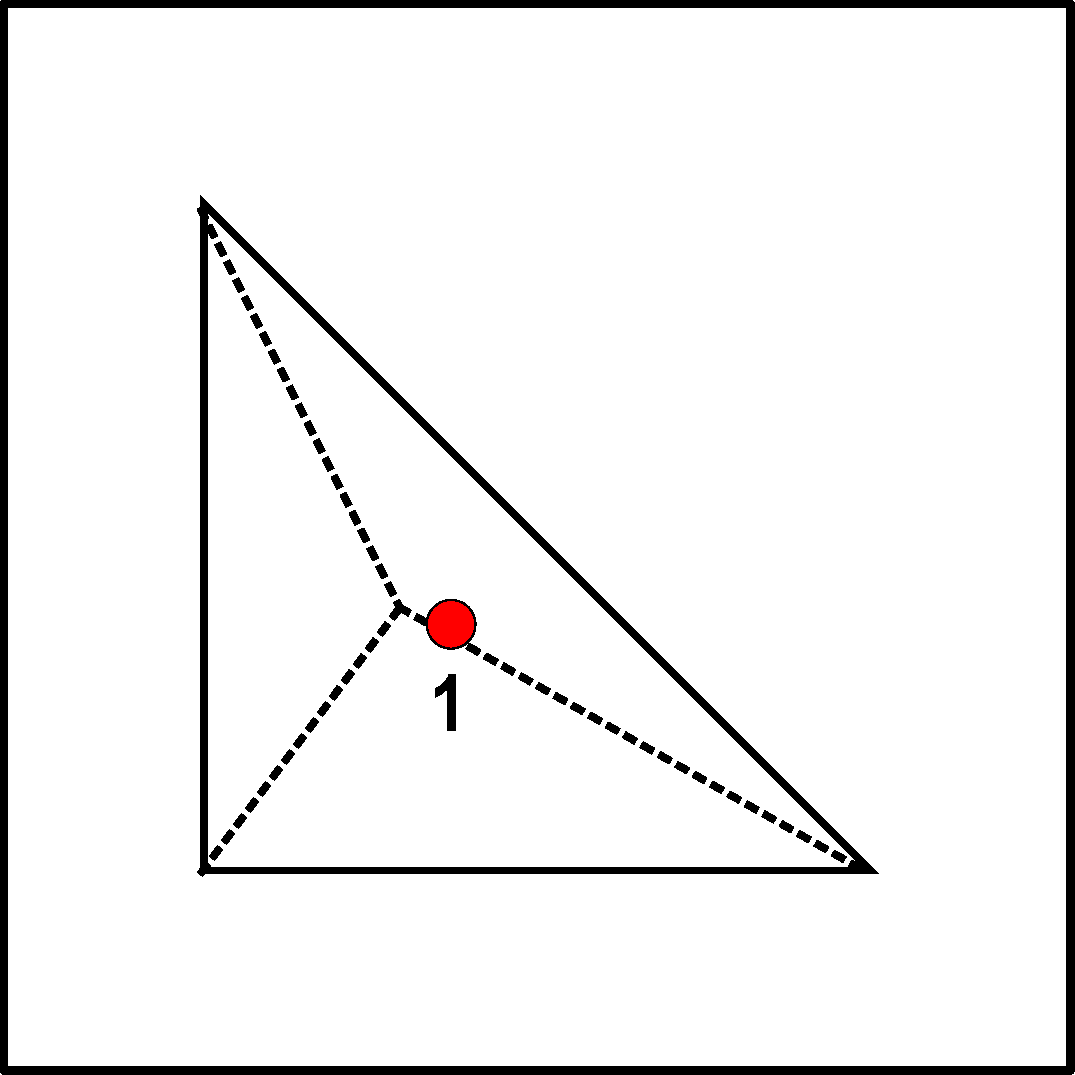
\includegraphics[width=2cm]{images/fe/p03d.pdf}}
\subfigure[$\mathbb{P}1$]{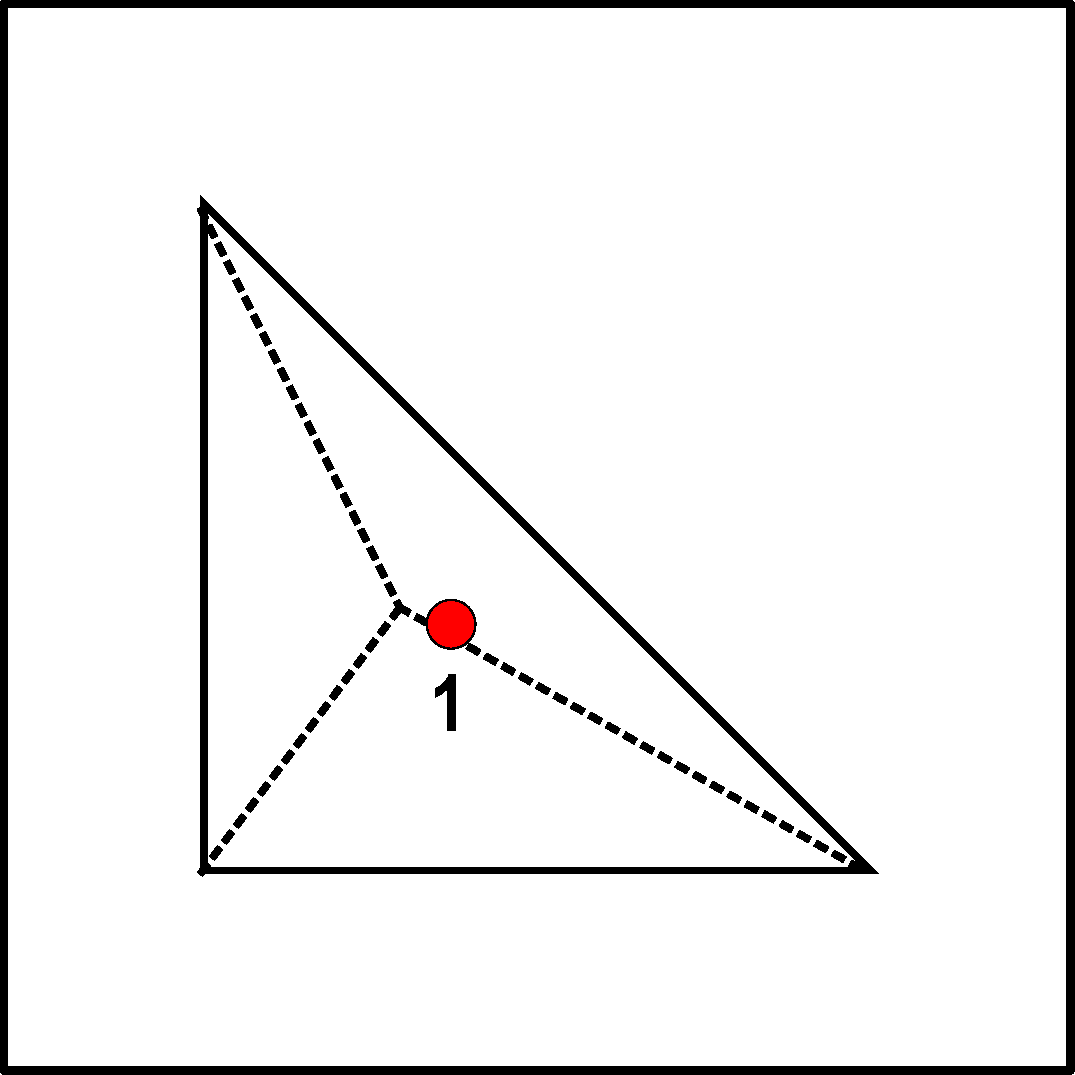
\includegraphics[width=2cm]{images/fe/p03d.pdf}}
\subfigure[$\mathbb{P}1$Bubble]{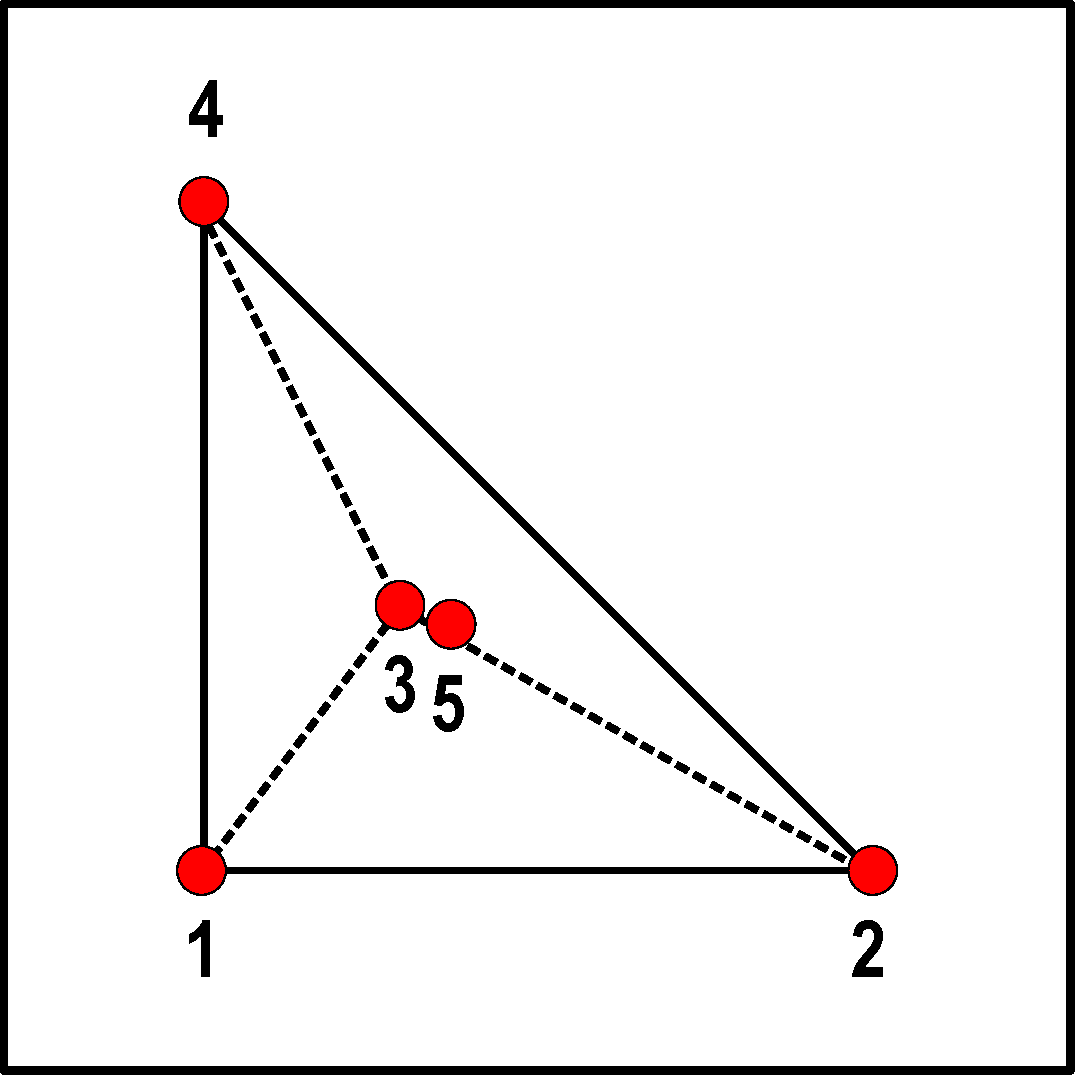
\includegraphics[width=2cm]{images/fe/P1Bubble3D.pdf}}
\subfigure[$\mathbb{P}2$]{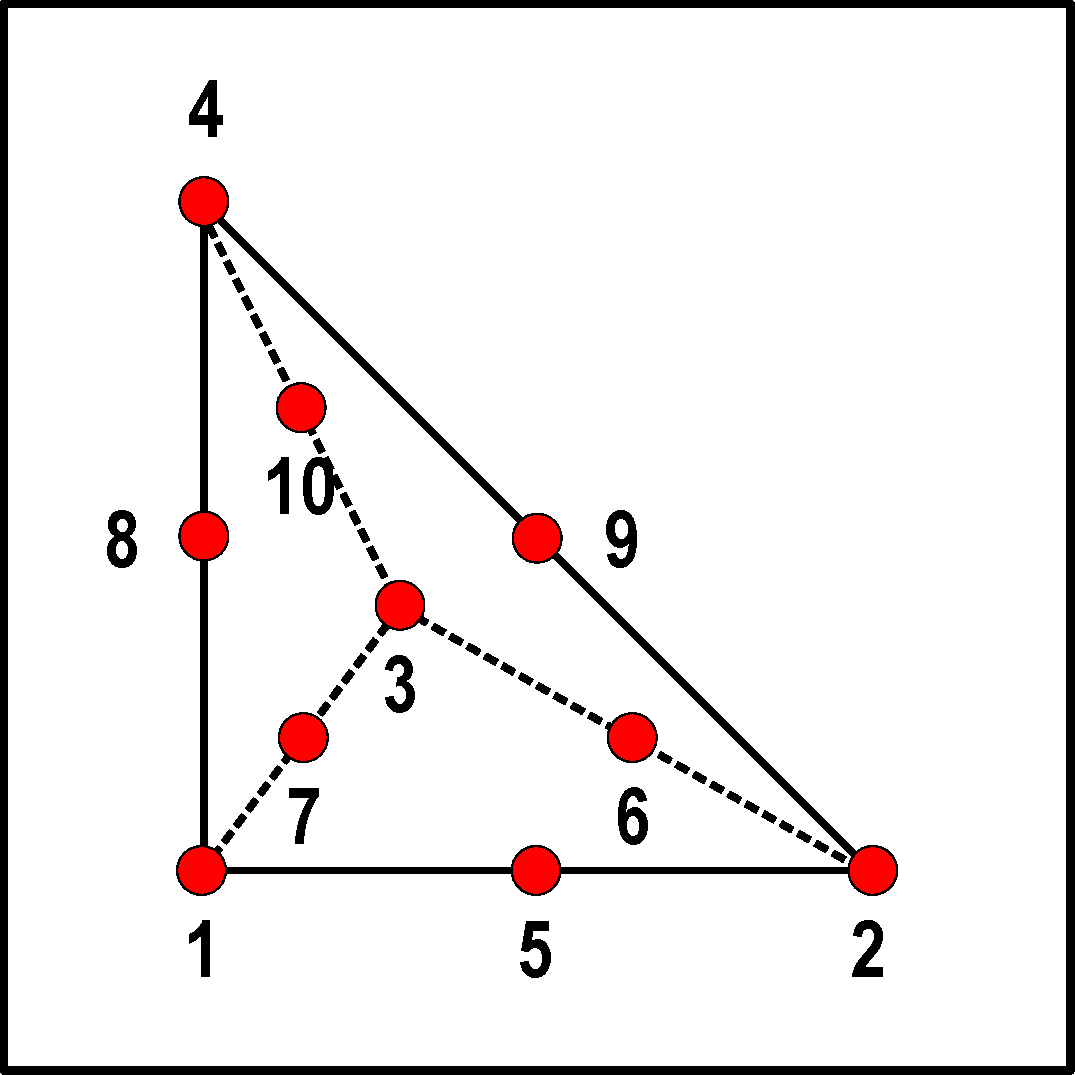
\includegraphics[width=2cm]{images/fe/p23d.pdf}}
\end{center}
\caption{Overview of the 3D finite elements available}
\label{fig:FE}
\end{figure}
Other elements and 2D elements are probably retrievable from LifeV-serial. Each finite element is an instance of the \texttt{RefFE} class.

%\begin{table}[H]
%\begin{center}
%\begin{tabular}{m{2cm}|m{2cm}m{2cm}m{2cm}m{2cm}}
% & \begin{center} 0D \end{center} & \begin{center} 1D \end{center} & \begin{center} 2D \end{center} & \begin{center} 3D \end{center} \\
%\hline
%$\mathbb{P}$0 & \includegraphics[width=2cm]{images/FE/P00D.pdf} &  \includegraphics[width=2cm]{images/FE/NA.pdf} & \includegraphics[width=2cm]{images/FE/P02D.pdf} & \includegraphics[width=2cm]{images/FE/P03D.pdf} \\
%$\mathbb{P}$1 & \includegraphics[width=2cm]{images/FE/NA.pdf} & \includegraphics[width=2cm]{images/FE/P11D.pdf} & \includegraphics[width=2cm]{images/FE/P12D.pdf} &  \includegraphics[width=2cm]{images/FE/P13D.pdf} \\
%$\mathbb{P}$1Bubble & \includegraphics[width=2cm]{images/FE/NA.pdf} & \includegraphics[width=2cm]{images/FE/NA.pdf} & \includegraphics[width=2cm]{images/FE/NA.pdf} &  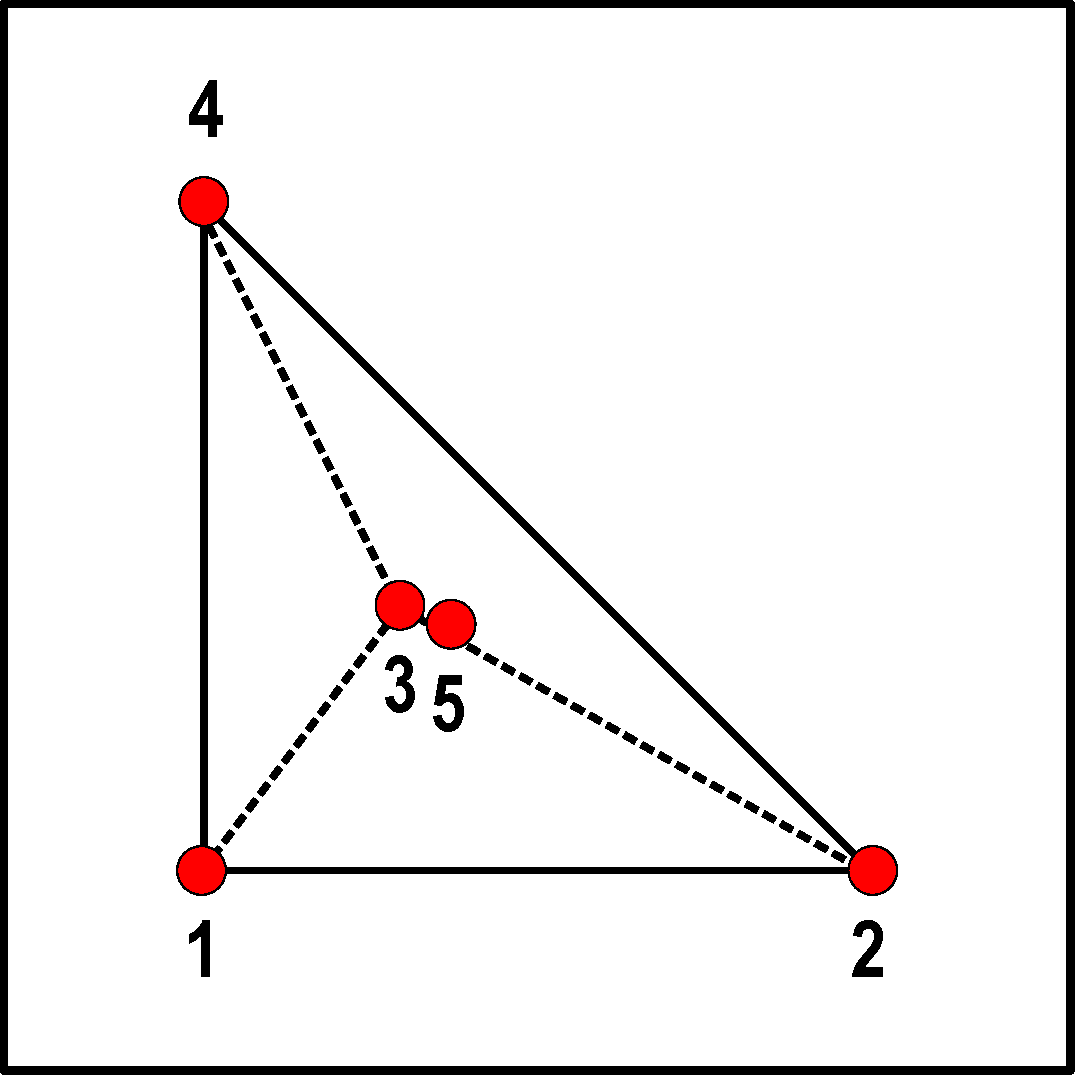
\includegraphics[width=2cm]{images/FE/P1Bubble3D.pdf} \\
%$\mathbb{P}$2 & \includegraphics[width=2cm]{images/FE/NA.pdf} & \includegraphics[width=2cm]{images/FE/P21D.pdf} & \includegraphics[width=2cm]{images/FE/P22D.pdf} &  \includegraphics[width=2cm]{images/FE/P23D.pdf} \\
%$\mathbb{P}$2tilde & \includegraphics[width=2cm]{images/FE/NA.pdf} & \includegraphics[width=2cm]{images/FE/NA.pdf} & \includegraphics[width=2cm]{images/FE/NA.pdf} &  \includegraphics[width=2cm]{images/FE/P2Tilde3D.pdf} \\
%RT0 & \includegraphics[width=2cm]{images/FE/NA.pdf} & \includegraphics[width=2cm]{images/FE/NA.pdf} & \includegraphics[width=2cm]{images/FE/NA.pdf} &  \includegraphics[width=2cm]{images/FE/RT0Tetra3D.pdf}
%\end{tabular}
%\end{center}
%\caption{Overview of the finite elements available}
%\end{table}
%The $\mathbb{P}$2tilde are Navier-Stokes $\mathbb{P}$2 basis oriented to the mass lumping.
%\begin{table}[H]
%\begin{center}
%\begin{tabular}{m{1cm}|m{2cm}m{2cm}}
% & \begin{center} 2D \end{center} & \begin{center} 3D \end{center} \\
%\hline
%$\mathbb{Q}$0 & \includegraphics[width=2cm]{images/FE/Q02D.pdf} & \includegraphics[width=2cm]{images/FE/Q03D.pdf} \\
%$\mathbb{Q}$1 & \includegraphics[width=2cm]{images/FE/Q12D.pdf} & \includegraphics[width=2cm]{images/FE/Q13D.pdf} \\
%$\mathbb{Q}$2 & \includegraphics[width=2cm]{images/FE/Q22D.pdf} & \includegraphics[width=2cm]{images/FE/NA.pdf} \\
%RT0 & \includegraphics[width=2cm]{images/FE/NA} & \includegraphics[width=2cm]{images/FE/RT0Hexa3D.pdf}
%\end{tabular}
%\end{center}
%\caption{Overview of the finite elements available}
%\end{table}

% Input/output in LifeV
\subsection{Input/output in LifeV}
\label{sec:inOutput}
Scientific computing involves a lot of data: Physical parameters, methods or solvers settings, meshes of the domain(s), output of the solution, $\ldots$

In this section we go through the different kind of input and output data used in LifeV.

\subsubsection{Input files}
The most common way to pass data to LifeV are data files containing parameters and values stored. The informations are then retrieved in the program using GetPot\footnote{More informations about the format and GetPot are available on http://getpot.sourceforge.net}.

\subsubsection{Mesh formats}
LifeV contains parsers to load mesh from the INRIA mesh (\texttt{.mesh}) format. The following formats are probably retrievable from LifeV-serial:
\begin{itemize}
\item Mpp mesh (\texttt{.m++});
\item Gmsh mesh (\texttt{.msh});
\item Netgen mesh (\texttt{.vol}).
\end{itemize}

\subsubsection{3D Structured mesh generator}
Instead of loading a mesh from a file, LifeV is able to generate a structured mesh with the function \texttt{structuredMesh3D}. This generator is useful to obtain quickly a mesh of a cuboid. One can also use it to obtain several refinements of a cuboid in order to evaluate the scalability of parallel algorithms or to test convergence rates on test problems.

\subsubsection{Output files}
When the computations are over, the user can collect the solution into output files. In the older versions of LifeV, the output were in the \texttt{vtk} format. The main disadvantage of this format is that each simulation generate hundreds of files!

In the new version, all the outputs are stored in one unique file in the \texttt{hdf5} format.

\subsubsection{Postprocessing}
Since the outputs are written in the \texttt{vtk} or in the \texttt{hdf5} format, many possibilities are available to use the results. However most of the LifeV's users use Paraview\footnote{More details are available on http://www.paraview.org}.

% Algorithms available in LifeV
\subsection{Algorithms available in LifeV}
LifeV does not only provide solvers but also tools and algorithms which helps to develop applications.

\subsubsection{GeneralizedAitken class}
\label{sec:aitken}
% Simone Deparis
This class is an implementation of the Aitken method which permits to compute automatically a relaxation parameter to accelerate the convergence of the fixed-point iterations. We give here a rough idea of the method. More details can be found in~\cite{deparis}.

Let $\mathbf{f}$ be a vector map from $\mathbb{R}^d$ to $\mathbb{R}^d$. We want to solve the fixed point problem $\mathbf{f}(\mathbf{x})=\mathbf{x}$, which can be rewritten as $\mathcal{R}(\mathbf{x})=\mathbf{f}(\mathbf{x})-\mathbf{x} = 0$. If $\mathbf{x}^k$ denotes the approximation of $\mathbf{x}$ at the step $k$ of the algorithm (with $\mathbf{x}^k\neq\mathbf{x}$), then $\mathcal{R}(\mathbf{x}^k)=\epsilon\neq0$. We want to calculate $\omega^k$ such that we can find a new approximation $\mathbf{x}^{k+1}=\mathbf{x}^k+\omega^k\mathcal{R}(\mathbf{x}^k)$ optimizing the convergence rate of the series~$\{\mathbf{x}^k\}$. More precisely, we have the following algorithm.

\begin{algorithme}[H]
\begin{enumerate}
\item Initial guess of $\mathbf{x}^0$ and $\omega^0$.
\item Set $\mathbf{x}^{k+1}=\mathbf{x}^k-\omega^k\mathcal{R}(\mathbf{x}^k)$
\item Compute $\mathcal{R}(\mathbf{x}^{k+1})$
\item \IfThenElse{$\norm{\mathcal{R}(\mathbf{x}^{k+1})}<\epsilon$}{
	Exit
}{
	Compute $\omega^{k+1}=\frac{(\mathcal{R}(\mathbf{x}^{k+1})-\mathcal{R}(\mathbf{x}^k))\cdot(\mathbf{x}^{k+1}-\mathbf{x}^k)}{\norm{\mathcal{R}(\mathbf{x}^{k+1})-\mathcal{R}(\mathbf{x}^k)}^2}$\\ $k=k+1$\\ Return to $2$.
}
\end{enumerate}
\caption{Aitken acceleration method}
\label{algoAitkenAccelerationMethod}
\end{algorithme}

\subsubsection{RCM reordering}
% Paolo Crosetto
This algorithm does a reordering of the nodes in such a way that the bandwidth of the matrix of the problem is minimized. The method is described in~\cite{saad}. The implemented code is tested via the test \texttt{test\_reorder}.

\subsubsection{Eigen values  computation}
% Paolo Crosetto
Using the Anazazi package from Trilinos\footnote{more informations available on http://trilinos.sandia.gov}, LifeV is able to compute eigen values from a matrix. In particular the test \texttt{test\_eigensolver} in the Mathcard testsuite compute the eigen values of a preconditioner.

% Meshes available in LifeV
\subsection{Meshes available in LifeV}
The LifeV release proposes lots of meshes like cylinders or cubes used in examples. A particular mesh available is a mesh of the carotid artery (see Figure~\ref{fig:carotidMesh}).

\begin{figure}[H]
\centering
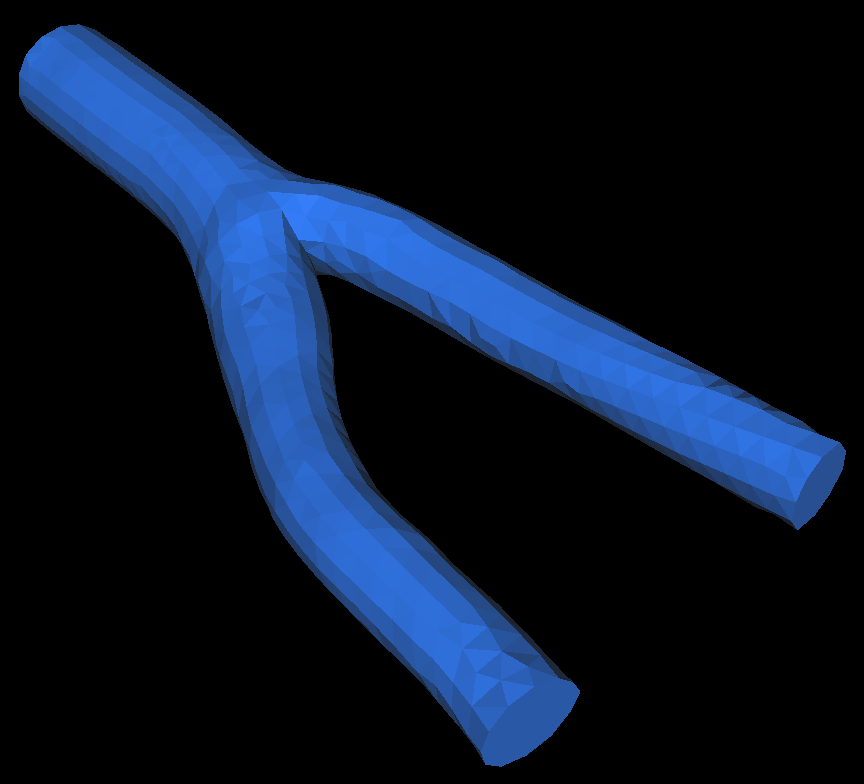
\includegraphics[width=6cm]{images/geometriesAndMeshes/carotid.png}
\caption{Mesh for blood flow simulations in the carotid artery}
\label{fig:carotidMesh}
\end{figure}

%============================
% Applications
%============================
\section{Applications}
\label{sec:applications}
In this section, we give an overview of the problem solved with LifeV.

% Convergence: Eithersteinman
\subsection{Convergence: Eithiersteinman}
% Simone Deparis, Gwenol Grandperrin
Eithier and Steinman have proposed an exact fully 3D Navier-Stokes solutions in~\cite{ethiersteinman}. This solution is used as a benchmark in LifeV to check the validity of the code.

% Multiscale models
\subsection{Multiscale models}
In the contexte of blood flows simulation, we want to be able to split the cardiovascular system into several pi�ces. Each of the pieces can be veins, artery or organs. Moreover to be able to compute such system we want to introduce a 1D model for the smallest vessels. So in the end we will make the computation on a general network of 1D or 3D problems where the edges will be the coupling and the nodes the problems. The details about the theory of this section can be found in~\cite{malossi}.

\subsubsection{Equations}
Currently, only the Oseen equations are available for the models in the network. Concerning the boundary conditions between the models one can choose between the two following possibilities:
\begin{enumerate}
\item flow-stress connection (see Figure~\ref{fig:multiscaleBCa});
\item stress-stress connection (see Figure~\ref{fig:multiscaleBCb}).
\end{enumerate}

\begin{figure}[H]
\centering
\subfigure[ ]{
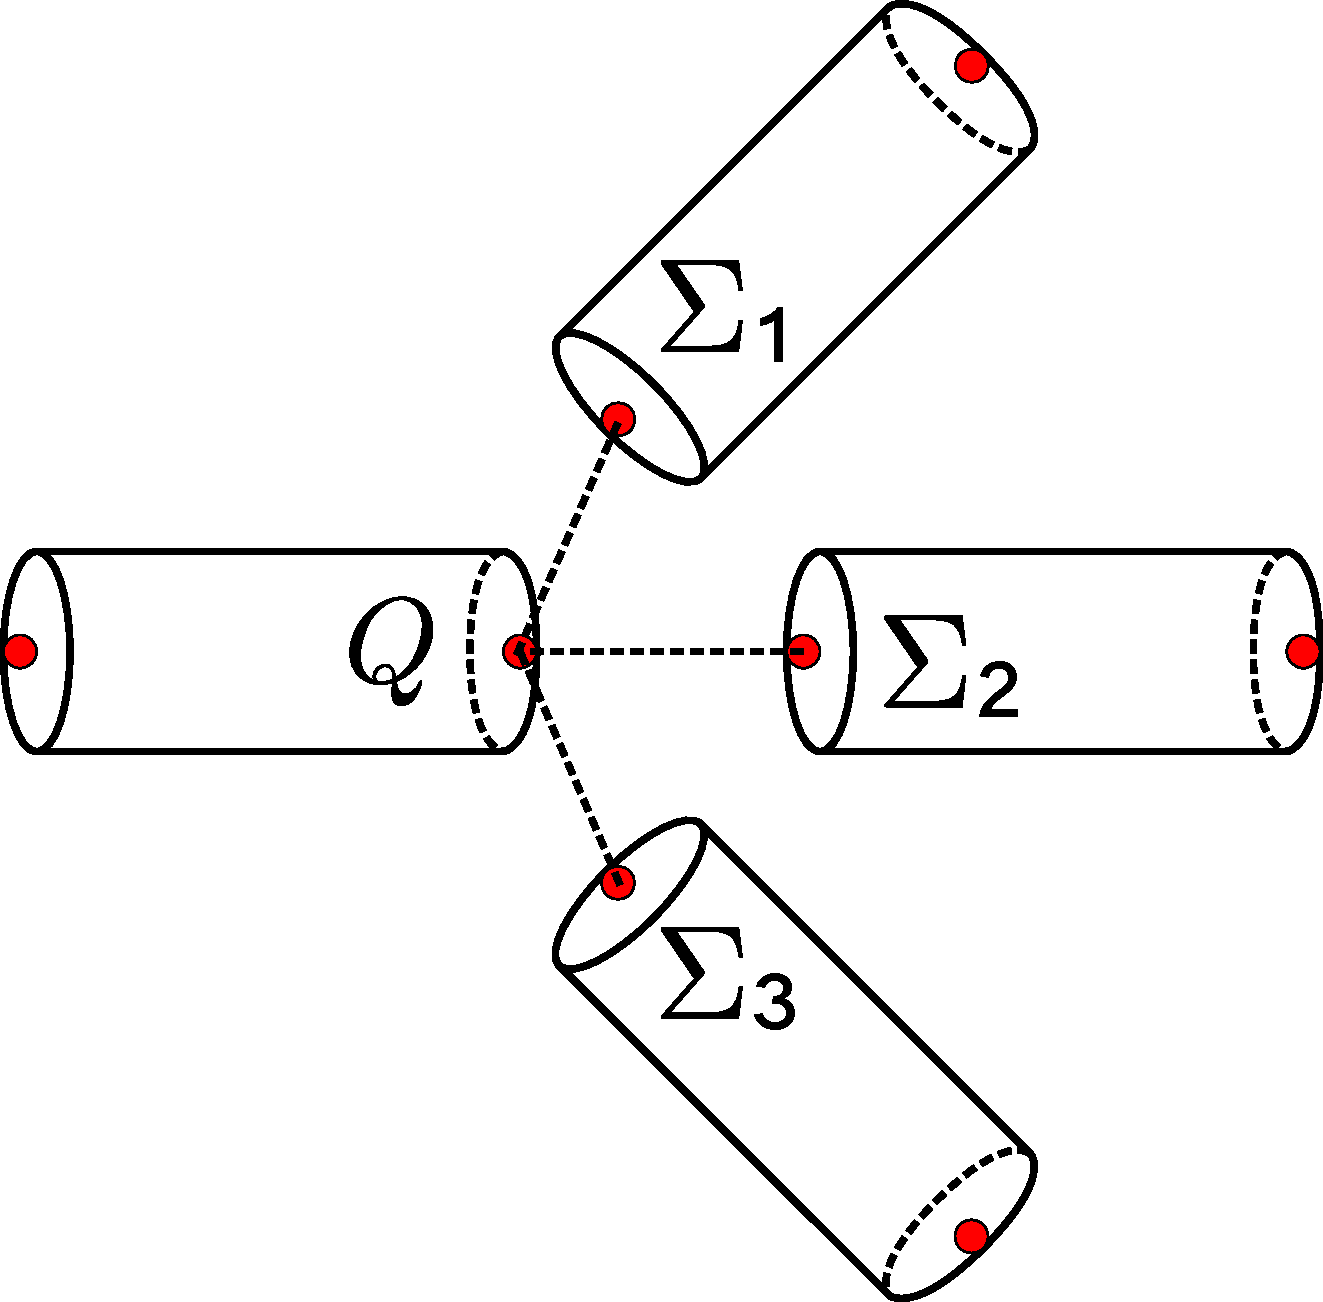
\includegraphics[width=4cm]{images/multiscale/bca.pdf}
\label{fig:multiscaleBCa}
}
\subfigure[ ]{
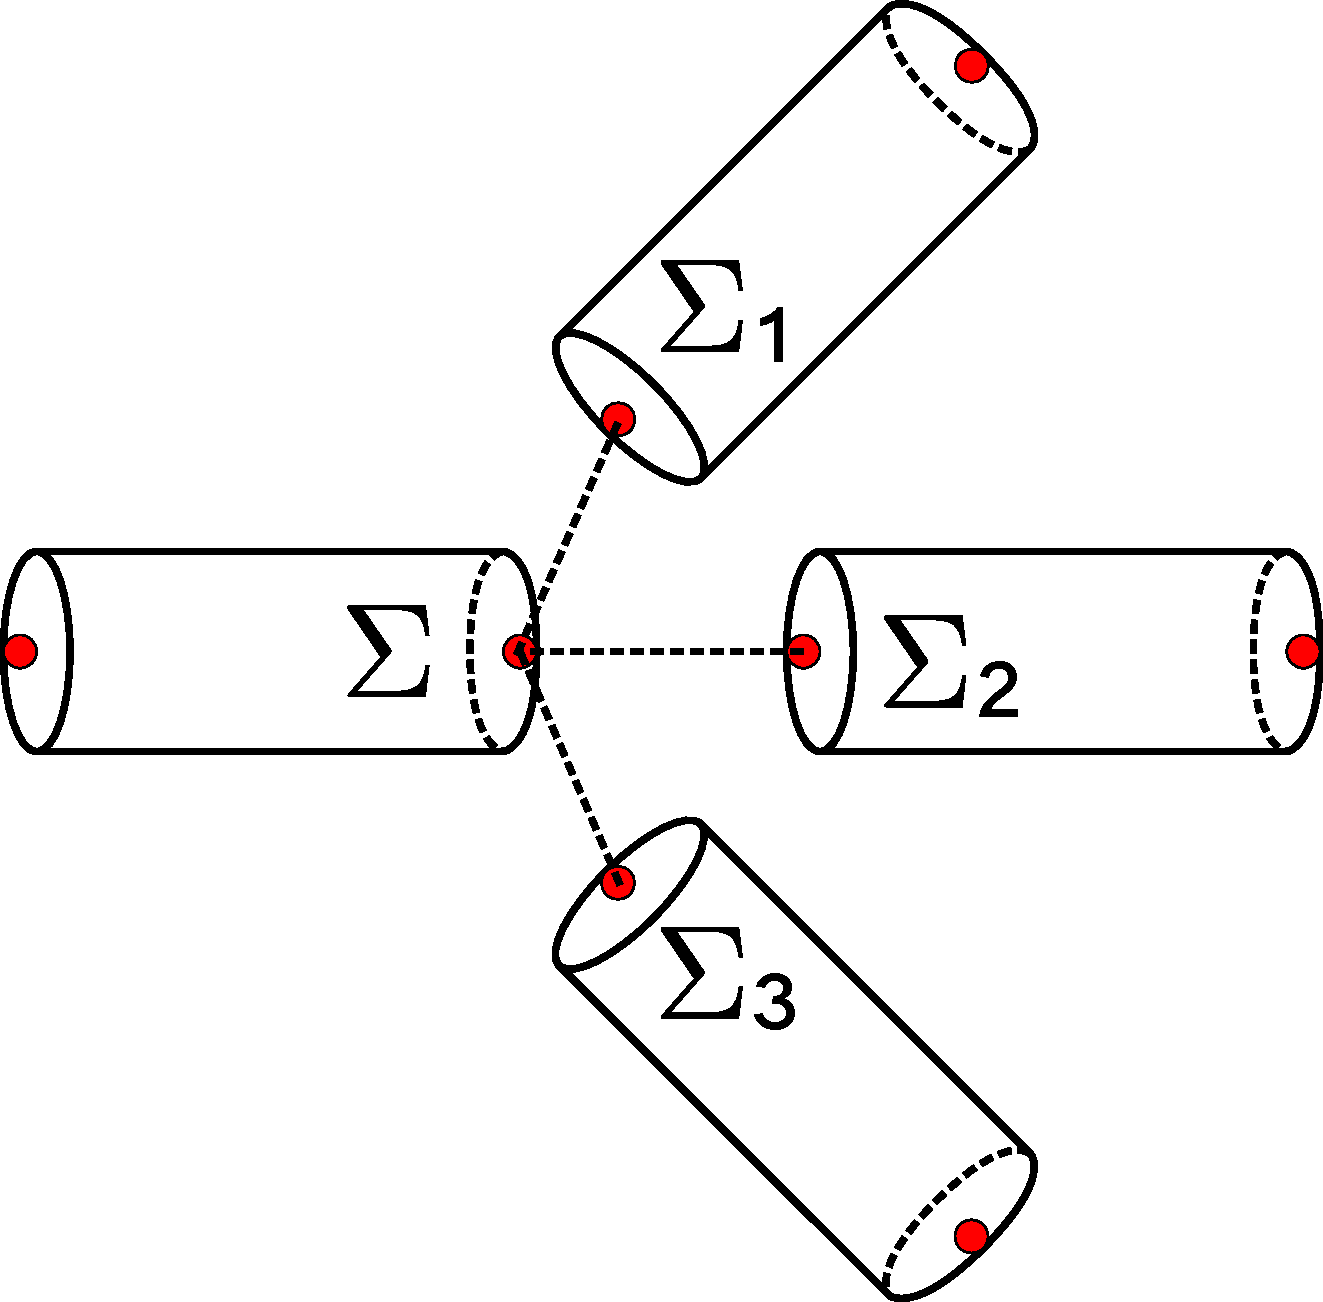
\includegraphics[width=4cm]{images/multiscale/bcb.pdf}
\label{fig:multiscaleBCb}
}
\caption{Explicit method}
\label{fig:multiscaleBC}
\end{figure}

If the stress and the flow are available the two possibilities are equivalent.

\subsubsection{Solving methods}
\begin{itemize}
\item Method 1 (Explicit):\\
This method only works with simple geometries (no bifurcations) and a very small time-step. We first solve the problem by imposing zero Neumann boundary condition at the coupling boundaries. At each time step, the information is propagated through the boundaries (see Figures~\ref{fig:multiscaleExplicitMethoda} to~\ref{fig:multiscaleExplicitMethodc}).
\begin{figure}[H]
\centering
\subfigure[t=0]{
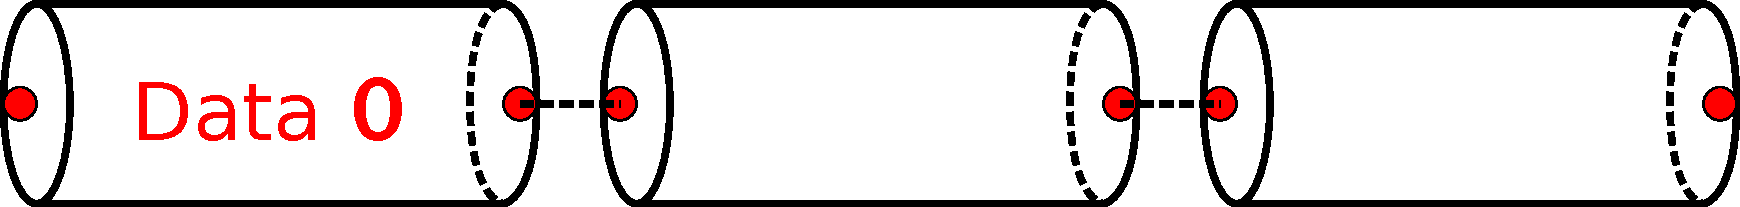
\includegraphics[width=7cm]{images/multiscale/explicitMethoda.pdf}
\label{fig:multiscaleExplicitMethoda}
}
\subfigure[t=1]{
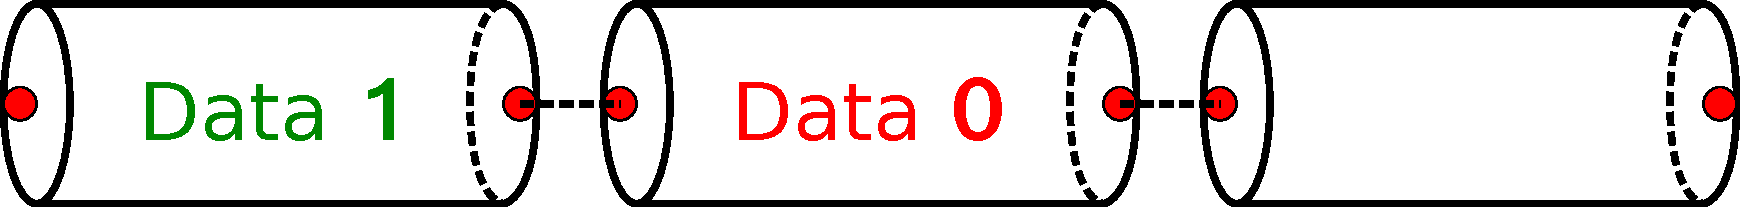
\includegraphics[width=7cm]{images/multiscale/explicitMethodb.pdf}
\label{fig:multiscaleExplicitMethodb}
}
\subfigure[t=2]{
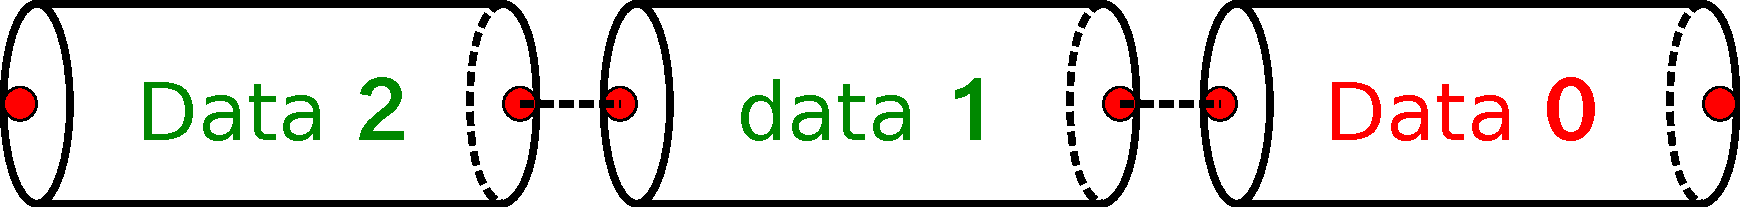
\includegraphics[width=7cm]{images/multiscale/explicitMethodc.pdf}
\label{fig:multiscaleExplicitMethodc}
}
\caption{Explicit method}
\label{fig:multiscaleExplicitMethod}
\end{figure}

\item Method 2 (implicit)\\
We use an implicit Aitken method (see Section~\ref{sec:aitken}) to solve the system. With this method, there is no limitation for $\Delta t$ due to the network. The evaluation of the residual make this method quite cheap. The method works fine with simple geometries but fails when bifurcations are introduced.

\item Method 3 (implicit)\\
We use an (implicit) Newton method to solve the system. We need to compute the jacobian, which is more expensive than the residual of Method 2.

\end{itemize}
Generally the solution is expensive, so it is better to reduce the number of iterations.


\subsubsection{Applications}
\begin{enumerate}
\item The first application is a network of five cylinders connected to create a continuous vessel. A sinusoidal flow rate is imposed at one extremity. We obtain a Wonersley profile. Moreover an exact solution is available for this  problem.
\begin{figure}[H]
\begin{center}
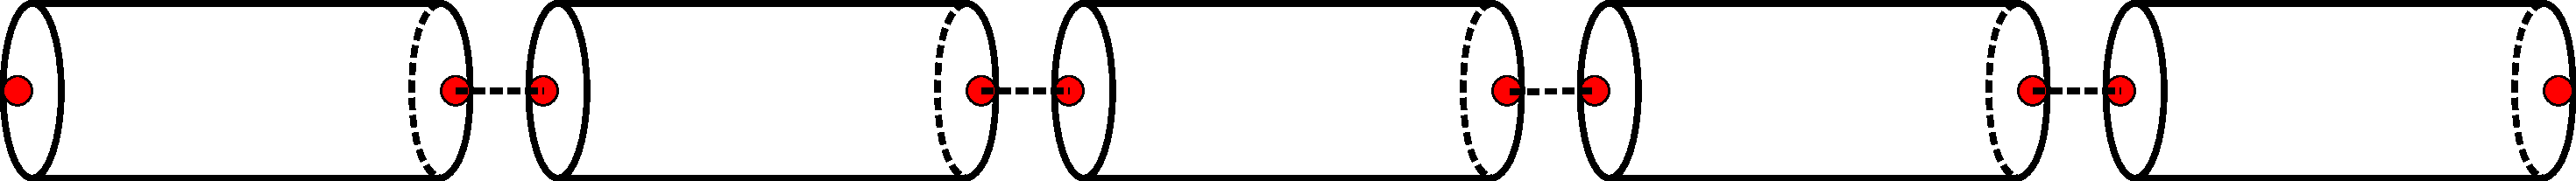
\includegraphics[width=8cm]{images/multiscale/application1.pdf}
\caption{Application 1}
\label{fig:multiscaleApplication1}
\end{center}
\end{figure}


\item In this application we introduce a bifurcation in the flow. This test allow to check if the flow is split correctly (the top and bottom branch should receive $\frac{1}{4}$ of the flow and the middle one $\frac{1}{2}$).
\begin{figure}[H]
\begin{center}
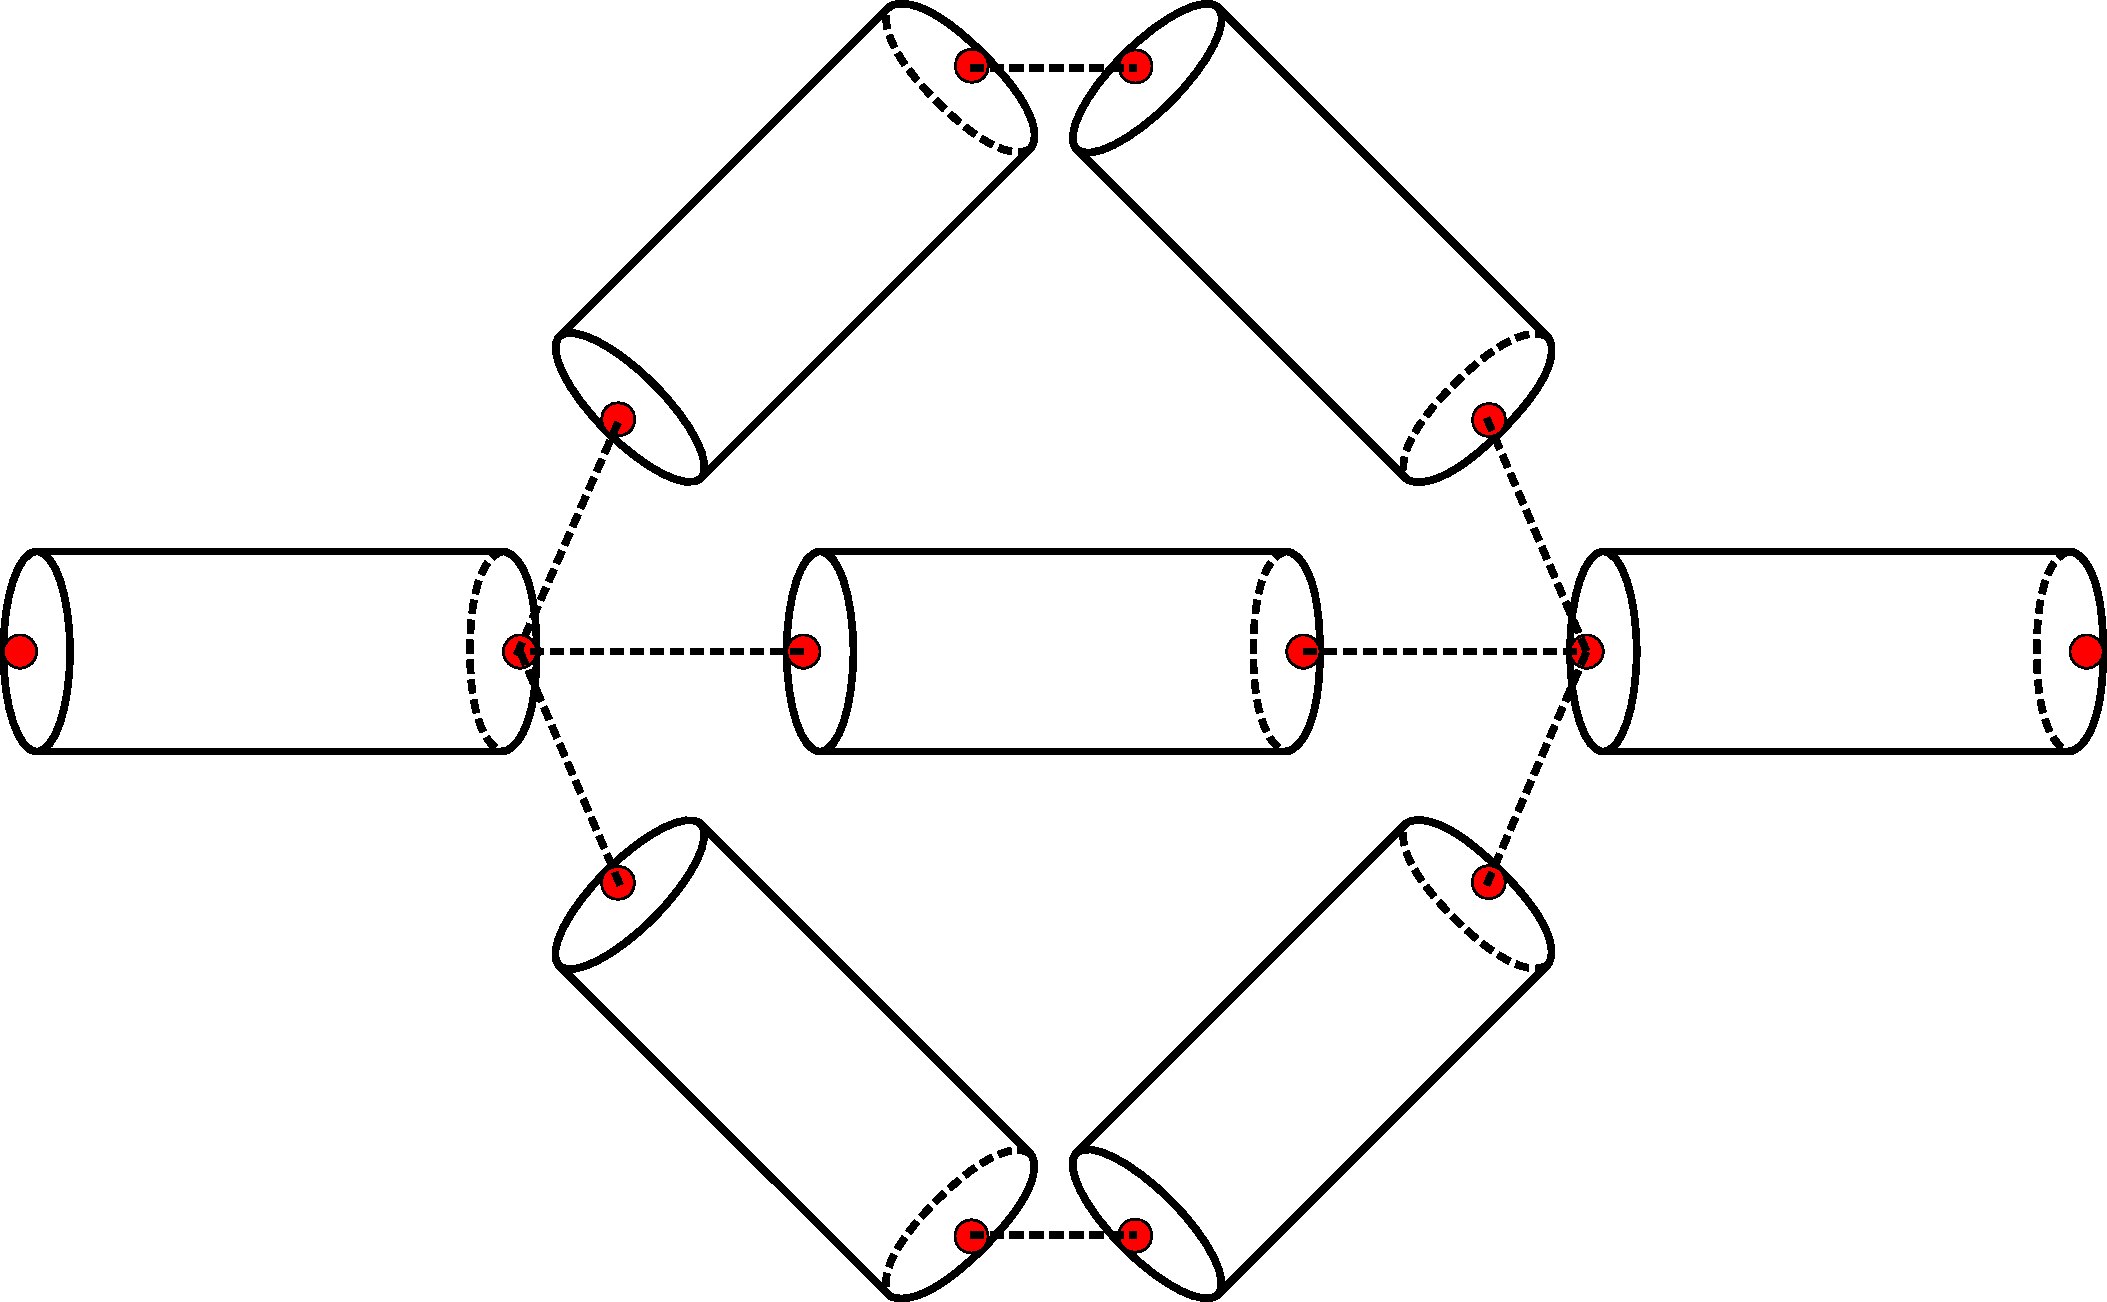
\includegraphics[width=6cm]{images/multiscale/application2.pdf}
\caption{Application 2}
\label{fig:multiscaleApplication2}
\end{center}
\end{figure}

\item We introduce a bifurcation in one of the models. Then we replace the bifurcation model by tree cylinders. We can then compare the accuracy of this substitution.

\begin{figure}[H]
\centering
\subfigure[ ]{
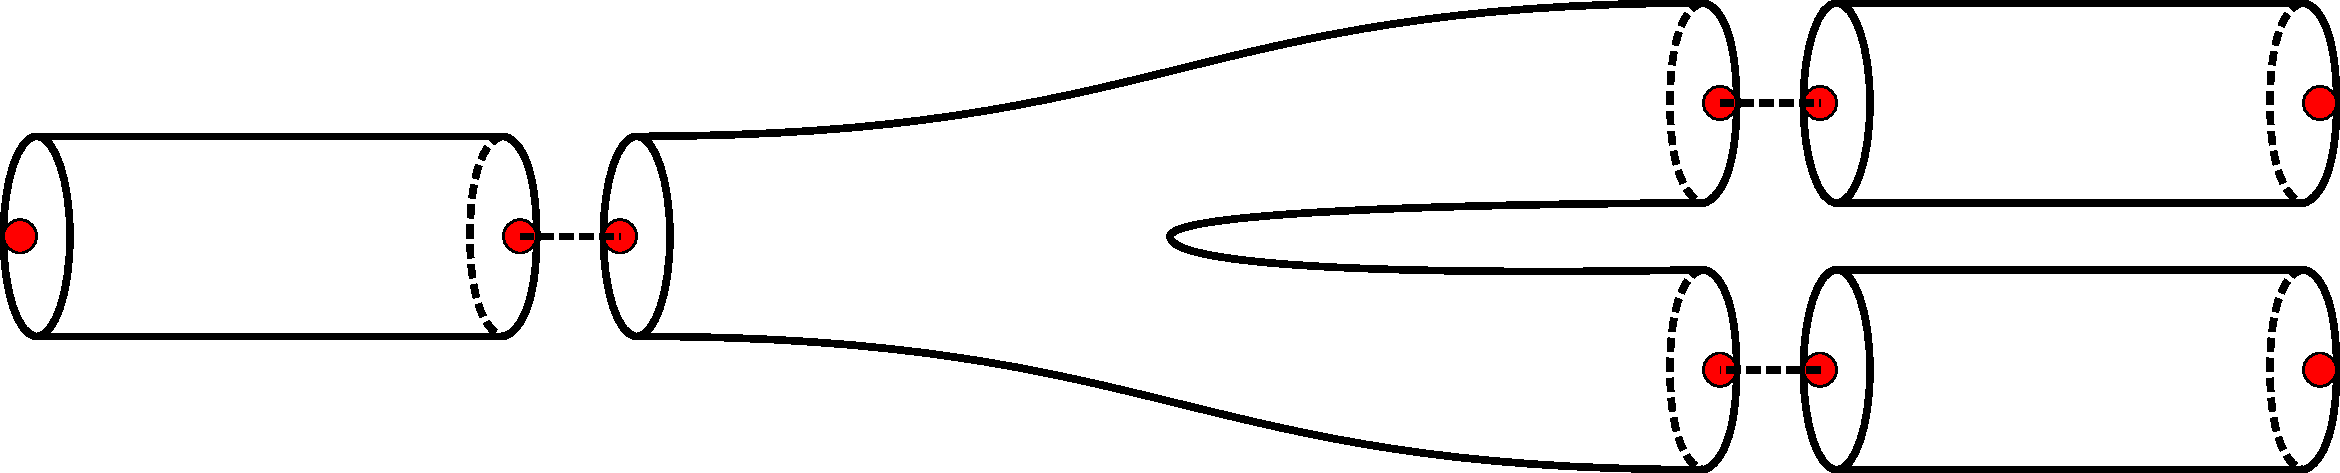
\includegraphics[width=7cm]{images/multiscale/application3a.pdf}
}
\subfigure[ ]{
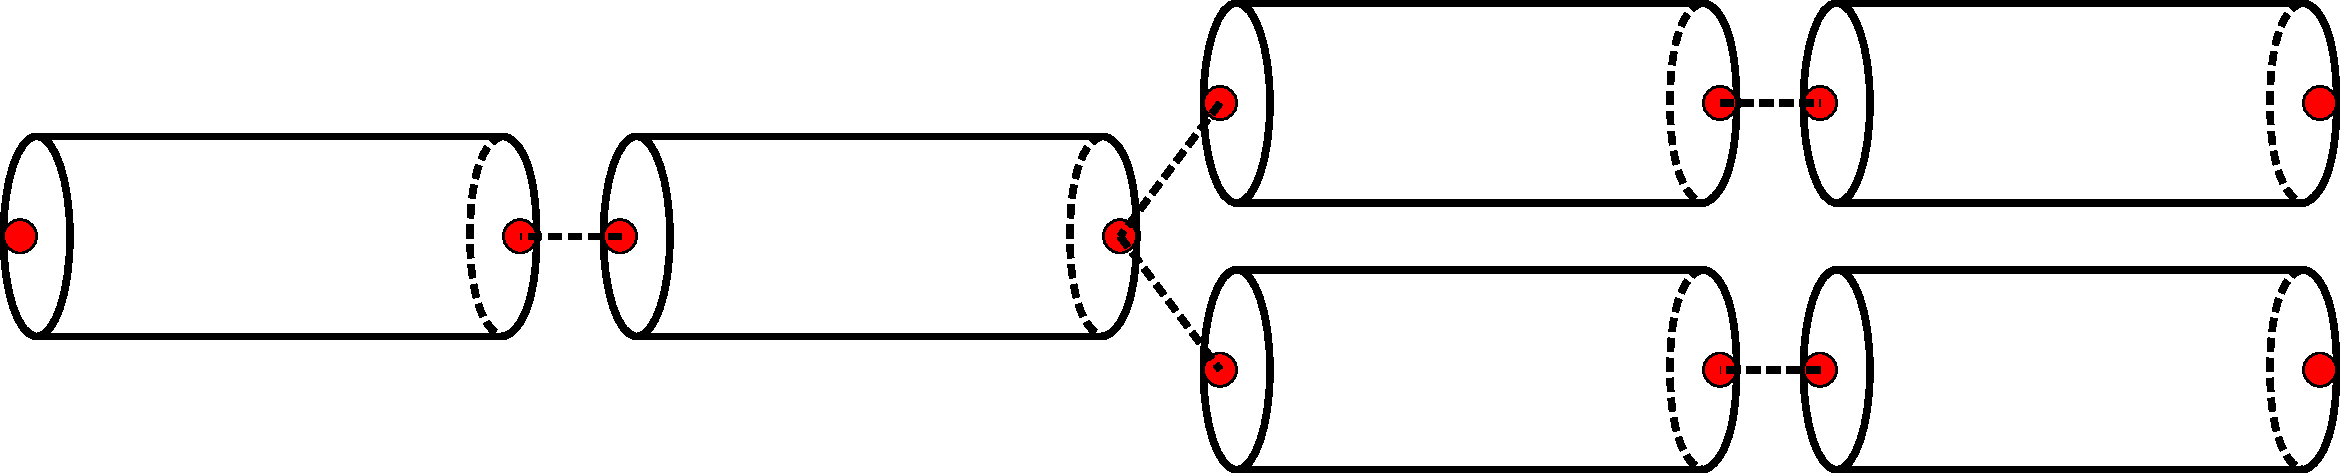
\includegraphics[width=7cm]{images/multiscale/application3b.pdf}
}
\caption{Application 3}
\label{fig:multiscaleApplication3}
\end{figure}

\end{enumerate}

\subsubsection{Future works}
Cristiano Malossi is currently working on the implementation of 1D models and their integration into the models network. He will also provide other solvers than Oseen for the models.

% Aorta with Fluid Structure Interaction (FSI) and delective BC
\subsection{Aorta with Fluid Structure Interaction (FSI) and delective BC}
% Paolo Crosetto
The theory concerning the resolution of FSI problem with parallel algorithm can be found in~\cite{crosetto}. A prior test is available (i.e. \texttt{test\_fsi}) which solves a FSI problem using the Newton method or an Aitken method. The convective term is treated explicitly but the geometry can be treated explicitly or implicitly.

A simulation of an aorta is done using Navier-Stokes (derived from the Oseen problem). It is available in \texttt{CMCS applications/application}.

\subsubsection{Future works}
A test of scalability for the simulation of the aorta with the FSI equations is under construction.

% Vessels deformation
\subsection{Vessels deformation}
% Paolo Tricerri & Margarita
An important aspect of blood flows simulation is the vessels deformation. Nonlinear elasticity solver is already implemented in LifeV with the Saint Venant-Kirchhof model (see Section~\ref{sec:venantKirchhofSolver}).

The \texttt{test\_nonlinearelasticity} test simulates the deformation of a cylinder. For this test we impose an homogenous Dirichlet boundary condition in the direction of the principal axis of the cylinder on $\Gamma_1$, an homogenous Neumann boundary condition on $\Gamma_2$ and a non homogenous Neumann boundary condition on $\Gamma_3$.

\begin{figure}[H]
\begin{center}
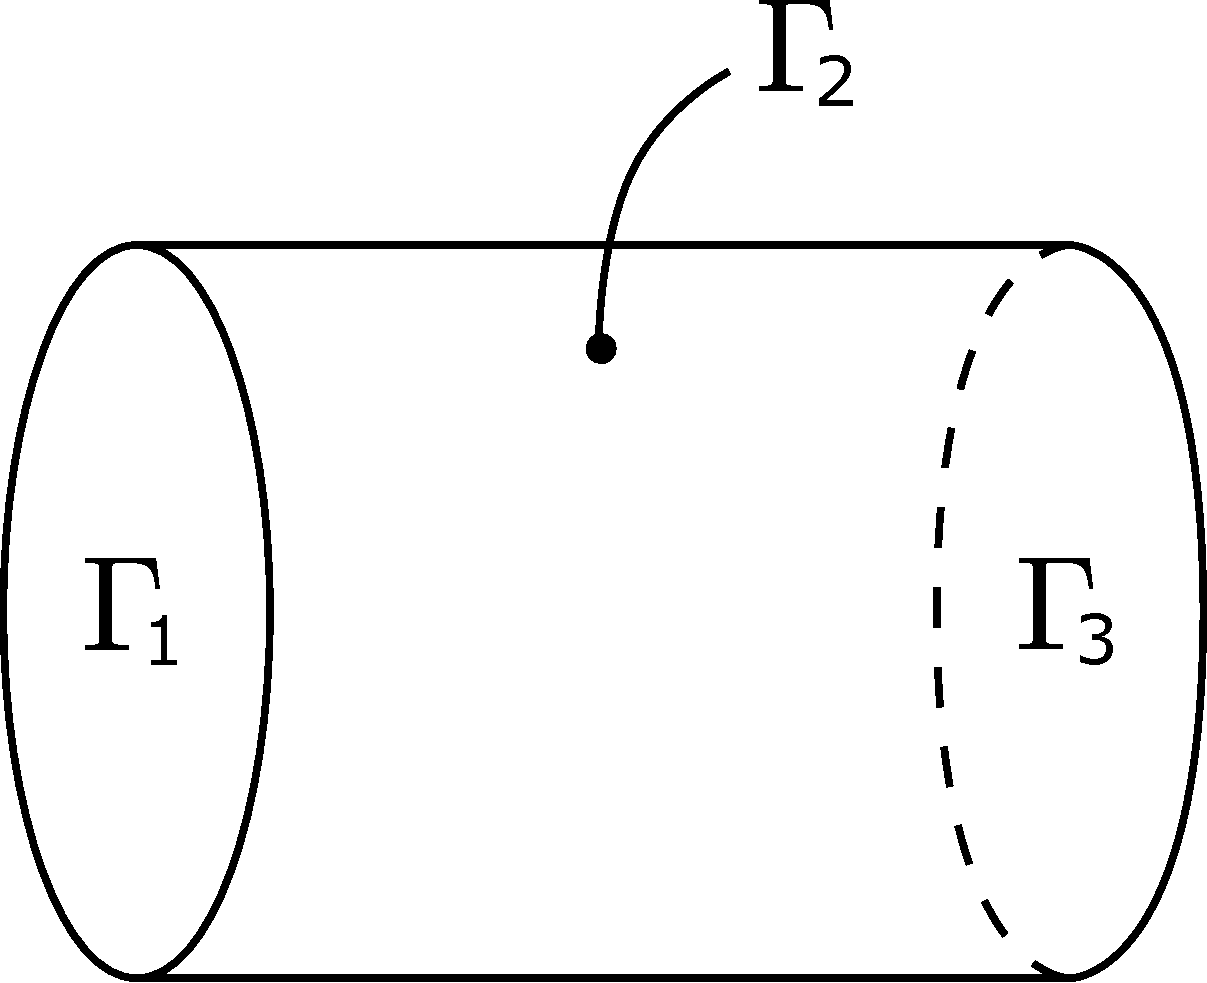
\includegraphics[width=4cm]{images/monolitic/cylindredomain.pdf}
\caption{Boundary conditions}
\label{fig:monoliticDomain}
\end{center}
\end{figure}

\subsubsection{Future works}
In the serial version of LifeV, others models exists and should be ported to LiveV:
\begin{enumerate}
\item The weakly exponential model;
\item The neo Hookean model.
\end{enumerate}
Moreover to obtain realistic model for the arterial wall deformation one should take into account the effects of elastin and collagen. Two tests (also in Life), \texttt{test\_structure\_1mec} and \texttt{test\_structure\_2mec}, take into account one or both substance respectively.

% Heart electrical propagation
\subsection{Heart electrical propagation}
\label{sec:heartElectricalPropagation}
% Ricardo Ruiz
A human heart is stimulated with electrical signals. In this application we try to simulate the electrical propagation.

A test case is available in the tests suite (i.e. \texttt{test\_heart}).

An interesting domain is the truncated ellipsoidal domain (see Figure~\ref{fig:truncatedEllipsoidalDomain}). Indeed the fibers description are known and the problem becomes non-linear for this geometry.
\begin{figure}[H]
\begin{center}
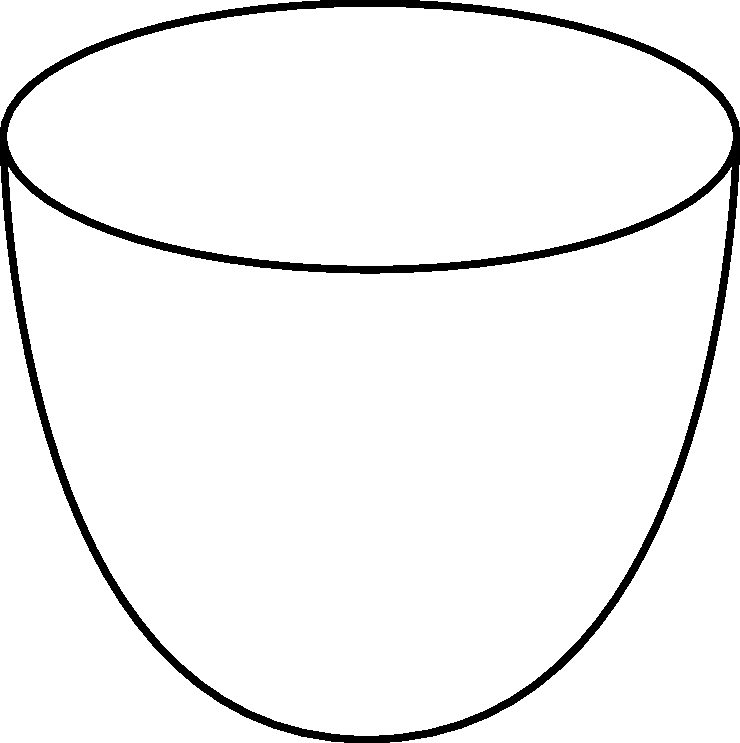
\includegraphics[width=4cm]{images/monoAndBidomain/truncatedellipsoidaldomain.pdf}
\caption{Truncated ellipsoidal domain}
\label{fig:truncatedEllipsoidalDomain}
\end{center}
\end{figure}

% 1D tree
\subsection{1D tree}
% Gilles Fourestey, Tiziano Passerini
The simulation of the entire cardiovascular system is very ambitious. A way to perform simulations is to consider a simple model: Each arteria, each vein and each capillary can be replaced by a 1D vessel. Putting all these models together we end up with a tree of vessels.


%============================
%============================
%============================


%============================
% Other projects
%============================
\section{Other projects}
\label{sec:otherProjects}
LifeV is not limited to an isolate development. Indeed several projects are currently involving the library:
\begin{itemize}
\item Mathcard project (EPFL-MOX)
\item Synergia
\end{itemize}
The following sections proposed an overview of the applications and current works related to the above projects.

% Monolitic (Mathcard)
\subsection{Monolitic (Mathcard)}
A \emph{monolitic} solver is implemented in LifeV. By \emph{monolitic} we mean that the solid and the fluid equations are solved in a unique matrix. The \texttt{test\_monolitic} tests a problem in a cylinder where the boundary are given in Figure~\ref{fig:monoliticDomain}. We impose an entering flux on $\Gamma_1$, Robin boundary condition on $\Gamma_2$ and absorbing Neumann boundary condition on $\Gamma_3$. The latter condition use Riemann invariant and the entering wave is imposed to $0$.
\begin{figure}[H]
\begin{center}
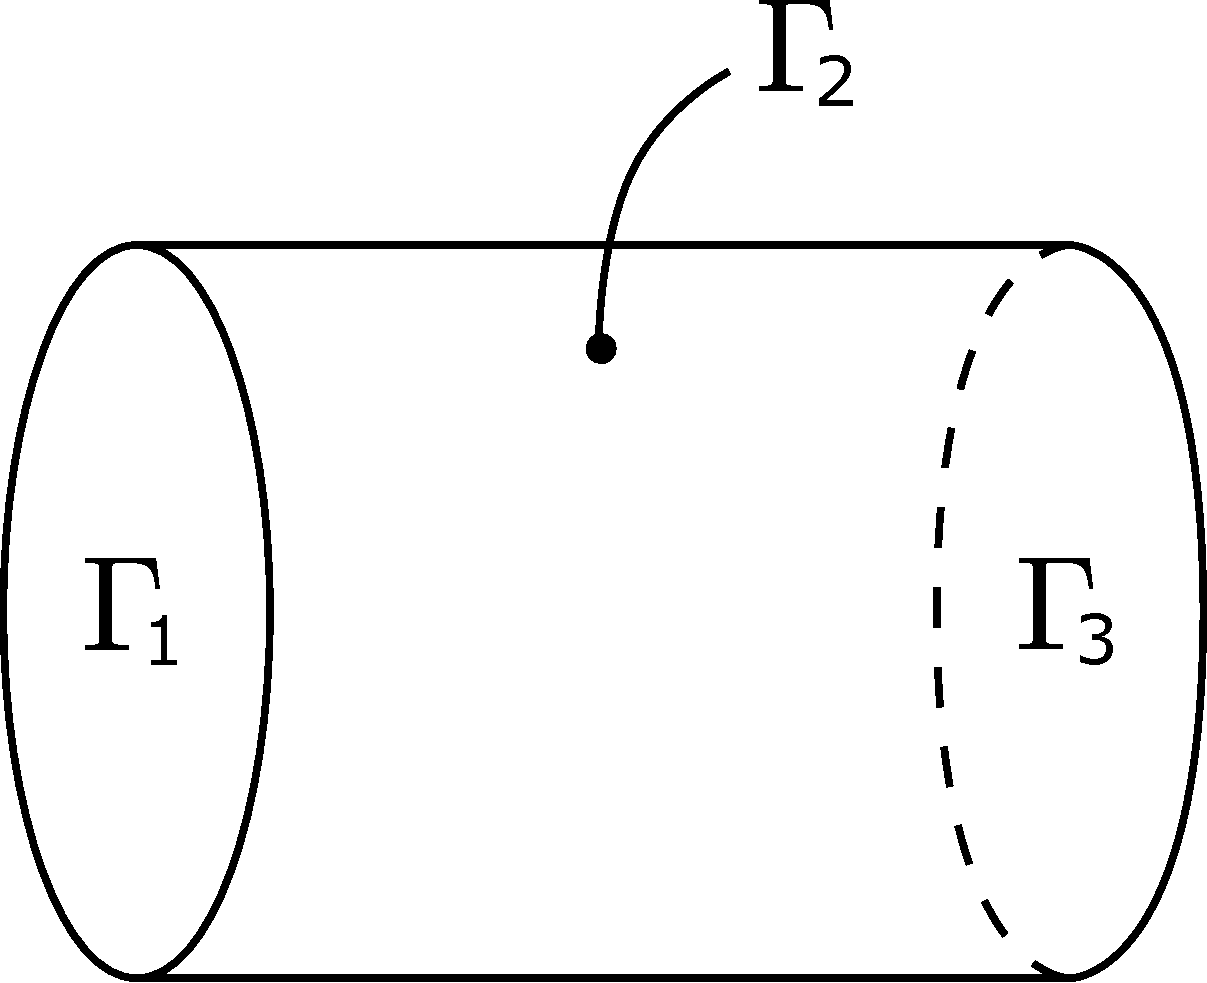
\includegraphics[width=4cm]{images/monolitic/cylindredomain.pdf}
\caption{Boundary conditions}
\label{fig:monoliticDomain}
\end{center}
\end{figure}

\subsubsection{Applications}
As an applications, a simulation of blood flow in the aorta has been made using the FSI equations (see Figure~\ref{fig:aortaFSISimulation}). This application is available in \texttt{CMCS applications/application}.

\begin{figure}[H]
\centering
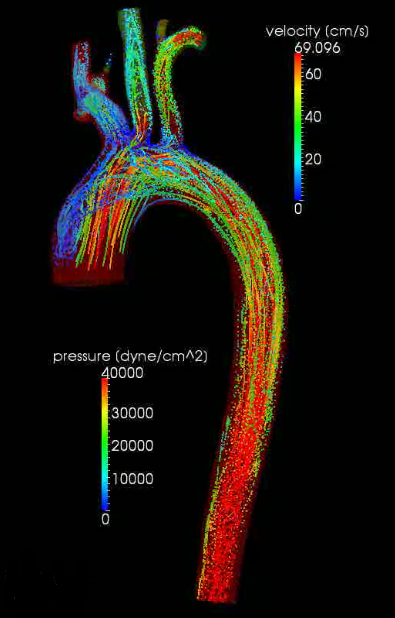
\includegraphics[height=10cm]{images/geometriesAndMeshes/crosettoAorta.png}
\caption{Aorta FSI simulation}
\label{fig:aortaFSISimulation}
\end{figure}

% Description of an electro-mechanic coupling
\subsection{Description of an electro-mechanic coupling (Mathcard)}
% Ricardo Ruiz
This application solves a problem composed by the equations~(\ref{eqn:MonoDomain1})-(\ref{eqn:MonoDomain2}) and the equation
\begin{equation}
-\nabla\cdot\sigma_{os}=0,
\end{equation}
where $\sigma_{os}$ is the Piola-Kirschhof tensor.
The implementation is given in the \texttt{test\_elecmech} test. However it is not ready yet.

% Physiological geometries/meshes (Mathcard)
\subsection{Physiological geometries/meshes (Mathcard)}
%1 - artery.vtp
%2 - bypass.vtp
%3 - aorta_angio_IRM_pelvis_bifurcations2_mc_c1.vtp
%4&5 - preop-afb.vtp
%6 - postop-afb.vtp
%7- virtual_aorta_1.vtp
%8 - palmaz-stent.vtp
%9 - palmaz-stent-expanded.vtp
%10 - heart.mesh
In order to do practical calculation, LifeV regrouped several physiological geometries for the Mathcard project. Since one of the practical interest is the simulation of the cardiovascular system, meshes simulating the vessels are available such as the bypass (proposed in~\cite{ku}) configuration where the blood flow is divided (see Figure~\ref{fig:vesselsGeometries1}), or an artery bifurcation (see Figure~\ref{fig:vesselsGeometries2}), or the aorta (proposed by \cite{simbios} and illustrated in~Figure~\ref{fig:vesselsGeometries3}).

\begin{figure}[H]
\centering
\subfigure[Bypass]{
\includegraphics[height=3.5cm]{images/geometriesAndMeshes/bypass.png}
\label{fig:vesselsGeometries1}
}
\subfigure[Artery]{
\includegraphics[height=3.5cm]{images/geometriesAndMeshes/artery.png}
\label{fig:vesselsGeometries2}
}
\subfigure[Aorta]{
\includegraphics[height=8cm]{images/geometriesAndMeshes/virtualAorta.png}
\label{fig:vesselsGeometries3}
}
\subfigure[Aorta bifurcations]{
\includegraphics[height=8cm]{images/geometriesAndMeshes/aortaIRM.png}
\label{fig:vesselsGeometries4}
}
\caption{Vessels geometries}
\label{fig:vesselsGeometries}
\end{figure}

The collection of geometries contains also particular situation like aneurysm geometry (before and after surgical operation, see Figures~\ref{fig:vesselsGeometries1} and~\ref{fig:vesselsGeometries2}; the two geometries are proposed in~\cite{wilson1} and~\cite{wilson2}) and medical device geometries like stents (compressed and extended version are showed on Figures~\ref{fig:vesselsGeometries3} and~\ref{fig:vesselsGeometries4}\footnote{Peter H. Feenstra of the Cardiovascular Biomechanics Research Laboratory at Stanford University is acknowledged for providing the geometry of the Palmaz-Schatz-like stent~(2006)}).

\begin{figure}[H]
\centering
%\subfigure[ ]{
%\includegraphics[width=4cm]{images/geometriesAndMeshes/preopAFB1.png}
%\label{fig:practicalInterestGeometries}
%}
\subfigure[Aneurysm before operation]{
\includegraphics[height=5cm]{images/geometriesAndMeshes/preopAFB2.png}
\label{fig:practicalInterestGeometries1}
}
\subfigure[Aneurysm after operation]{
\includegraphics[height=5cm]{images/geometriesAndMeshes/postopAFB.png}
\label{fig:practicalInterestGeometries2}
}
\subfigure[Palmaz stent]{
\includegraphics[height=3.7cm]{images/geometriesAndMeshes/stent.png}
\label{fig:practicalInterestGeometries3}
}
\subfigure[Palmaz extended stent]{
\includegraphics[height=3.7cm]{images/geometriesAndMeshes/stentExpanded.png}
\label{fig:practicalInterestGeometries4}
}
\caption{Practical interest of geometries}
\label{fig:practicalInterestGeometries}
\end{figure}

Of course as presented in Section~\ref{sec:heartElectricalPropagation}, simulations can also target phenomena on organs like the heart (see Figure~\ref{fig:heartMesh}).

\begin{figure}[H]
\centering
\subfigure[Front view]{
\includegraphics[height=5cm]{images/geometriesAndMeshes/heartfront.png}
\label{fig:heartMesh1}
}
\subfigure[Top view]{
\includegraphics[height=5cm]{images/geometriesAndMeshes/hearttop.png}
\label{fig:heartMesh2}
}
\caption{Mesh for the simulation of the heart}
\label{fig:heartMesh}
\end{figure}

% Levelset (Synergia/bioreactor)
\subsection{Level set (Synergia/bioreactor)}
% Samuel Quinodoz
The management of a level set function has been introduced in LifeV for the Synergia project. The aim is to simulate a bioreactor. The levelset is used to follow the deformation of the fluid in a tank full of water and nutrients.

Let us consider a partition $\Omega_1(t)$, $\Omega_2(t)$ of a domain $\Omega(t)$ (which can depend on the time $t$) and let $\Gamma_I$ denotes the interface between the two subsets. The level set method describes the interface as the zero level set of a function $\phi$:

\begin{equation}
\label{levelsetfct}
\left\{ \begin{array}{ll}
\phi(\mathbf{x},t) > 0 & \mathbf{x}\in\Omega_1(t)\\
\phi(\mathbf{x},t) < 0 & \mathbf{x}\in\Omega_2(t)\\
\phi(\mathbf{x},t) = 0 & \mathbf{x}\in\Gamma_I(t)
\end{array}\right.
\end{equation}
so that
\begin{equation}
\Gamma_I(t) = \{\mathbf{x}\in\Omega(t)\mid\phi(\mathbf{x},t)=0\}.
\end{equation}

Let $H$ be the Heavyside function defined by
\begin{equation}
\label{heavysidefct}
H(z)=
\left\{ \begin{array}{ll}
0 & z<0\\
1 & z>0
\end{array}\right. ,
\end{equation}
such that the density and the viscosity quantities in $\Omega$ can be rewritten as
\begin{equation}
\label{heavysidefct}
\begin{array}{ll}
\rho = \rho_1+(\rho_2-\rho_1)H(z)\\
\mu = \mu_1+(\mu_2-\mu_1)H(z)
\end{array}.
\end{equation}

The final system that describes the evolution of the fluid is composed of the Navier-Stokes equations~(\ref{eqn:NS1}) and~(\ref{eqn:NS2}) as well as the equation~(\ref{eqn:levelset}).
\begin{equation}
\label{eqn:levelset}
\begin{array}{ll}
\frac{\partial\phi}{\partial t}+\mathbf{u}\cdot\nabla\phi = 0 & \text{in }\Omega\times[0,T]\\
\phi=\phi_0 & \text{in }\Omega\text{ at }t=0\\
\phi=\phi_{in} & \text{on }\partial\Sigma_{in}\times[0,T]
\end{array}
\end{equation}
where $\Sigma_{in} = \{(\mathbf{x},t)\in\partial\Omega\times(0,T)\mid\mathbf{u}(\mathbf{x},t)\cdot\mathbf{n}<0\}$.

The main advantages of this method is that the interface remains sharp and handle any change in the topology of $\Gamma_I$. However it has drawbacks such as the distorsion of the interface caused by the numerical errors. To overcome this problem, one should use reinitialization of the interface.

\subsubsection{Level set solver}
The level set solver solves the equations~(\ref{eqn:levelset}). It manages also the reinitialization of the interface by using the geometric approach. Methods to compute the surface and the volumes of the domains  and to export the interface are available (only for $\phi$ approximate with $\mathbb{P}1$ finite element).

From the coding point of view, the level set solver is a class which inheritates from the AdvectionDiffusionReaction solver.

\subsubsection{OseenTwoFluids solver (not yet ready)}
This solver handles two fluids in a container. The separation of the fluids is made with the level set method.

\subsubsection{Applications}
\begin{enumerate}
\item The first application is actually a test to check the accuracy of the method. We take a prism with a circular basis. We draw a circle in the domain (see Figure~\ref{fig:levelsetTesta}). Then we set a velocity to rotate the circle (see Figure~\ref{fig:levelsetTestb}). After a few time steps, we set the velocity in the other direction. Finally we check if the circle came back at the initial position or if some error appears  (see Figure~\ref{fig:levelsetTestc}).
\begin{figure}[H]
\centering
\subfigure[t=0]{
\includegraphics[width=3.5cm]{images/levelset/levelsetTesta.pdf}
\label{fig:levelsetTesta}
}
\subfigure[t=1]{
\includegraphics[width=3.5cm]{images/levelset/levelsetTestb.pdf}
\label{fig:levelsetTestb}
}
\subfigure[t=2]{
\includegraphics[width=3.5cm]{images/levelset/levelsetTestc.pdf}
\label{fig:levelsetTestc}
}
\caption{Levelset test}
\label{fig:levelsetTest}
\end{figure}

\item The second application use the OseenTwoFluids to simulate a shaked cylindrical tank filled with two non-miscible fluids. However this application is not yet ready.
\end{enumerate}

\subsubsection{Future works}
As already mentioned, a new method for the reinitialization must be implemented in order to get better accuracy and computational cost. Moreover the OseenTwoFluids must be finished. One can also think about adapting the methods of the level set solver for other finite elements than $\mathbb{P}1$.

%=============================
% Conclusion
%=============================
\section{Conclusion}
In this document we have made an overview of the LifeV library state of the art. We have first presented the library itself. We described the physical solvers class available and heir main methods. We also presented the boundary conditions and the finite element implemented. We listed the input/output options provided by the library.

Then we presented a gallery of LifeV applications and projects which shows the flexibility and the possibilities of LifeV.

Finally we should recall that the LifeV developers continues to develop the code in order to achieves larger and more complex simulations on tomorrow's supercomputers.

%=============================
% Bibliographie
%=============================
\newpage
%index et bibliographie
%\printindex
\nocite{*}
\bibliography{biblio}
\bibliographystyle{plain}


\end{document}
